\PassOptionsToPackage{xetex}{xcolor}
\PassOptionsToPackage{xetex}{graphicx}
\documentclass[a4paper,landscape,headrule,footrule,xetex]{foils}

%%
%%%  Macros
%%%
\newcommand{\logo}{~}
\MyLogo{HG2052 (2021)}
%\newcommand{\Story}{\SHA{HOUN}{The Hound of the Baskervilles}}

\newcommand{\header}[3]{%
\title{\vspace*{-2ex} \Large HG2052
\\\large  Language, Technology and the Internet
\\[2ex] \Large  \emp{#2}}
\author{\blu{Francis Bond}   \\ 
\normalsize  \textbf{Division of Linguistics and Multilingual Studies}\\
\normalsize  \url{http://www3.ntu.edu.sg/home/fcbond/}\\
\normalsize  \texttt{bond@ieee.org}}
\MyLogo{HG2052 (2021); CC BY 4.0}
\date{#1}
\renewcommand{\logo}{#2}
 \hypersetup{
   pdfinfo={
     Author={Francis Bond},
     Title={#1: #2},
     Subject={HG2052: Language, Technology and the Internet},
     Keywords={Language, Technology, Internet},
     License={CC BY 4.0}
   }
 %  pdfcopyright={Copyright © Francis Bond. Creative Commons 4.0 Attribution License.}
 %  pdflicenseurl={http://creativecommons.org/licenses/by/4.0/}
 }
}

 %% must load before bidi
\usepackage[xetex]{xcolor} 
\usepackage[hidelinks]{hyperref}
\usepackage{natbib}
\usepackage{rtrees,qtree}
\newcommand{\lf}[1]{\br{#1}{}}


%%
%% Multilingual Stuff
%%
\usepackage[a4paper,landscape,margin=25mm]{geometry}

\usepackage{fontenc}
\usepackage{polyglossia}
\setmainlanguage{english}
\setmainfont{TeX Gyre Pagella}
%\setmainfont{Linux Libertine}
%\setmainfont{Charis SIL}
\newfontfamily{\ipafont}{Gentium}
\newcommand{\ipa}[1]{{\ipafont\selectfont #1}}
\usepackage{xeCJK}

\setCJKmainfont{Noto Sans CJK SC}
\setCJKsansfont{Noto Sans CJK SC}
%\setCJKttfont{Noto Sans CJK SC}
%\setCJKmainfont{WenQuanYi Micro Hei}
%\clearpage
%\setCJKmainfont{AR PL SungtiL GB}

%\newfontfamily\arabicfont[Script=Arabic]{Scheherazade}

\usepackage[xetex]{graphicx}
\newcommand{\blu}[1]{\textcolor{blue}{#1}}
\newcommand{\grn}[1]{\textcolor{green}{#1}}
\newcommand{\hide}[1]{\textcolor{white}{#1}}
\newcommand{\emp}[1]{\textcolor{red}{#1}}
\newcommand{\txx}[1]{\textbf{\textcolor{blue}{#1}}}
\newcommand{\lex}[1]{\textbf{\mtcitestyle{#1}}}

\usepackage{pifont}
\renewcommand{\labelitemi}{\textcolor{violet}{\ding{227}}}
\renewcommand{\labelitemii}{\textcolor{purple}{\ding{226}}}

\newcommand{\subhead}[1]{\noindent\textbf{#1}\\[5mm]}

\newcommand{\Bad}{\emp{\raisebox{0.15ex}{\ensuremath{\mathbf{\otimes}}}}}
\newcommand{\bad}{*}

\newcommand{\com}[1]{\hfill \textnormal{(\emp{#1})}}%
\newcommand{\cxm}[1]{\hfill \textnormal{(\txx{#1})}}%
\newcommand{\cmm}[1]{\hfill \textnormal{(#1)}}%
\usepackage{amssymb}
\usepackage{relsize,xspace}
\newcommand{\into}{\ensuremath{\rightarrow}\xspace}
\newcommand{\ent}{\ensuremath{\Rightarrow}\xspace}
\newcommand{\nent}{\ensuremath{\not\Rightarrow}\xspace}
\newcommand{\tot}{\ensuremath{\leftrightarrow}\xspace}
\usepackage{url}
\hypersetup{
     colorlinks,
     linkcolor={blue!50!black},
     citecolor={red!50!black},
     urlcolor={blue!80!black}
}
%\usepackage{hyperxmp}
\usepackage{url}
\newcommand{\lurl}[1]{\MyLogo{\url{#1}}}

\usepackage{mygb4e}
\let\eachwordone=\itshape
\newcommand{\lx}[1]{\textbf{\textit{#1}}}
\newcommand{\ix}{\ex\it}

\newcommand{\cen}[2]{\multicolumn{#1}{c}{#2}}
%\usepackage{times}
%\usepackage{nttfoilhead}
\newcommand{\myslide}[1]{%
\foilhead[-25mm]{\raisebox{12mm}[0mm]{\emp{#1}}}%
\leftheader{}%
\MyLogo{\logo}}

\newcommand{\mytask}[1]{%
\foilhead[-25mm]{\raisebox{12mm}[0mm]{\emp{#1}}}
\leftheader{🔍 Hi}%
\MyLogo{\logo}}

\newcommand{\myslider}[1]{\rotatefoilhead[-25mm]{\raisebox{12mm}[0mm]{\emp{#1}}}}
%\newcommand{\myslider}[1]{\rotatefoilhead{\raisebox{-8mm}{\emp{#1}}}}

\newcommand{\section}[1]{\myslide{}{\begin{center}\Huge \emp{#1}\end{center}}}

\usepackage{tcolorbox}
% \newcommand{\task}{\marginpar{\raisebox{-1ex}{\large
%       \tcbox[colframe=red,colback=white,arc=3pt]{\textbf{?}}}}}
% \newcommand{\task}{\marginpar{\raisebox{-1ex}{
%       \hspace{-0.5em}\tcbox[colframe=red,colback=white,arc=3pt]{%
%         \includegraphics[width=1.5em]{pics/detective}}}}}
\newcommand{\task}{\marginpar{\raisebox{-2ex}{
      \hspace{-0.5em}\reflectbox{\includegraphics[width=2em]{pics/detective}}}}}

\usepackage[lyons,j,e,k]{mtg2e}
\renewcommand{\mtcitestyle}[1]{\textcolor{teal}{\textsl{#1}}}
%\renewcommand{\mtcitestyle}[1]{\textsl{#1}}
\newcommand{\chn}{\mtciteform}
\newcommand{\cmn}{\mtciteform}
\newcommand{\iz}[1]{\textup{\texttt{\textcolor{blue}{\textbf{#1}}}}}
\newcommand{\con}[1]{\textsc{#1}}
\newcommand{\gm}{\textsc}
\newcommand{\cmp}[1]{{[\textsc{#1}]}}
\newcommand{\sr}[1]{\ensuremath{\langle}#1\ensuremath{\rangle}}
\usepackage[normalem]{ulem}
\newcommand{\ul}{\uline}
\newcommand{\uul}{\uuline}
\newcommand{\wl}{\uwave}
\newcommand{\vs}{\ensuremath{\Leftrightarrow}~}
%%%
%%% Bibliography
%%%
%\usepackage{url}
\usepackage{bibentry}


%%% From Tim
\newcommand{\WMngram}[1][]{$n$-gram#1\xspace}
\newcommand{\infers}{$\rightarrow$\xspace}



\usepackage{avm}
%\avmoptions{topleft,center}
\newcommand{\ft}[1]{\textsc{#1}}
%\newcommand{\val}[1]{\textit{#1}}
\newcommand{\typ}[1]{\textit{#1}}
\avmfont{\sc}
%\avmvalfont{\sc}
\renewcommand{\avmtreefont}{\sc}
\avmsortfont{\it}


%%% From CSLI book
\newcommand{\mc}{\multicolumn}
\newcommand{\HD}{\textbf{H}\xspace}
\newcommand{\el}{\< \>}
\makeatother
\long\def\smalltree#1{\leavevmode{\def\\{\cr\noalign{\vskip12pt}}%
\def\mc##1##2{\multispan{##1}{\hfil##2\hfil}}%
\tabskip=1em%
\hbox{\vtop{\halign{&\hfil##\hfil\cr
#1\crcr}}}}}
\makeatletter

\newcommand{\sh}[1]{\href{https://www.arthur-conan-doyle.com/index.php?title=#1}{#1}}
\newcommand{\SHA}[2]{\href{https://www.arthur-conan-doyle.com/index.php?title=#1}{\textit{#2}}}




\header{Lecture 10}{The Semantic Web}

\begin{document}

\bibliographystyle{apalike}
\nobibliography{abb,mtg,nlp,ling}

\maketitle


%\input{schedule}

\section{Revision of Text and Meta-text}
\myslide{Text and Meta-text}

\MyLogo{and Zombies}
\begin{itemize}
\item Explicit Meta-data
  \begin{itemize}
  \item Keywords and Categories
  \item Rankings
  \item Structural Markup
  \end{itemize}
\item Implicit Meta-data
  \begin{itemize}
  \item Links and Citations
  \item Tags
  \item Tables
  \item File Names
  \item Translations
  \end{itemize}
\end{itemize}

\myslide{Explicit Metadata}
\MyLogo{}
\begin{itemize}
\item You can get information from metadata within documents
  \begin{itemize}
  \item When they are accurate they are very good
  \item They are often deceitful
  \end{itemize}
\item HTML, PDF, Word, \ldots Metadata
\item Keywords and Tags
\item Rankings
\item Links and Citations
\item Structural Markup
\end{itemize}

\myslide{Implicit Metadata}
\begin{itemize}
\item You can get clues from metadata within documents
  \begin{itemize}
  \item as they are non-intended, they tend to be noisy
  \item but they are rarely deceitful
  \end{itemize}
\item HTML tags as constituent boundaries
\item Tables as Semantic Relations
\item File Names (content type and language)
\item Translations ---  Bracketed Glosses;  Cross-lingual Disambiguation
\item Query Data
\item Wikipedia Redirections and Cross-wiki Links
\end{itemize}

\section{The Semantic Web}


\myslide{The Semantic Web}

\begin{itemize}
\item What is it?
\item How is it built?
\item Why is it being built?
\item Problems
\end{itemize}

\myslide{The Semantic Web}

\begin{itemize}
\item A vision of a more useful World Wide Web
\item the meaning of information and services on the web is defined
\item machines (and people) can understand the web
\end{itemize}

\begin{center}
  \large The Web as a universal medium for \\ data, information, and knowledge exchange.
\end{center}

%%
%% FIXME
%%
%

\myslide{The Web as it is now}

\begin{itemize}
\item Resources
  \begin{itemize}
  \item Identified by URLs (uniform resource locator)
  \item Untyped
  \end{itemize}
\item Links
  \begin{itemize}
  \item href, src, \ldots
  \item limited, non-descriptive
  \end{itemize}
\item Human User
  \begin{itemize}
  \item Exciting World - Semantics deduced from context
  \end{itemize}
\item Machine User
  \begin{itemize}
  \item Very little explicit information
  \end{itemize}
\end{itemize}
\newpage

\myslide{The Current Web}
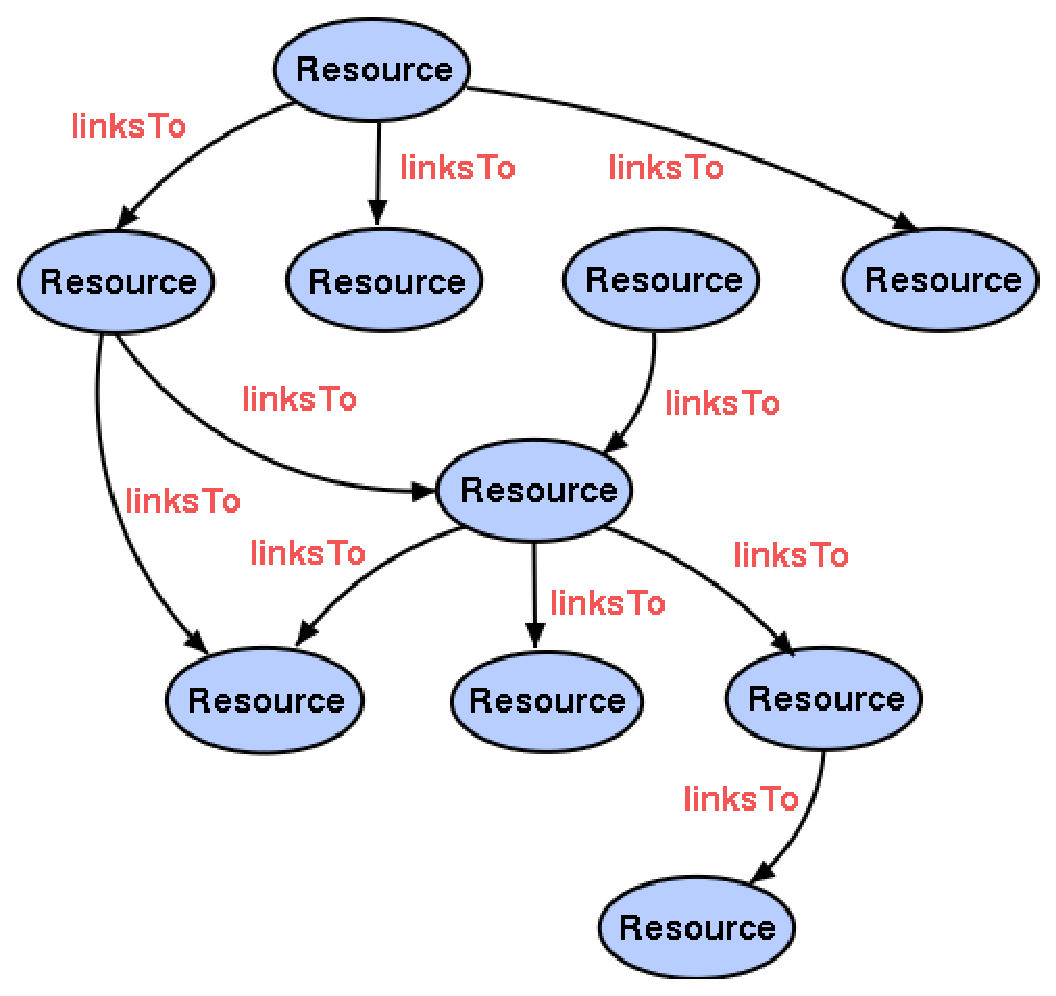
\includegraphics[height=\textheight]{../pics/currentweb.eps}



\myslide{The Web as it could be}

\begin{itemize}
\item Resources
  \begin{itemize}
  \item Globally Identified by URIs (uniform resource identifier)
  \item Extensible, Relational
  \end{itemize}
\item Links
  \begin{itemize}
  \item \emp{Identified by URIs}  \hfill \blu{Use the web to define the web}
  \item Extensible, Relational
  \end{itemize}
\item Human User
  \begin{itemize}
  \item Even more exciting world - Richer user experience
  \end{itemize}
\item Machine
  \begin{itemize}
  \item More processable information
  \end{itemize}
\end{itemize}
\newpage

\myslide{The Semantic Web}
\includegraphics[height=\textheight]{../pics/semanticweb.eps}

\myslide{Semantic Web Goals}

\begin{itemize} 
\item Web of Data
  \begin{itemize}
  \item provides common data representation framework
  \item makes possible integrating multiple sources
  \item so you can draw new conclusions
  \end{itemize}
\item  Increase the utility of information by connecting it to definitions and context
\item  More efficient information access and analysis
\end{itemize}

E.G. not just "color" but a concept denoted by a Web identifier: 
\\ \url{<http://en.wikipedia.org/wiki/Sapphire_(color)>}


\myslide{Semantic Web Architecture}

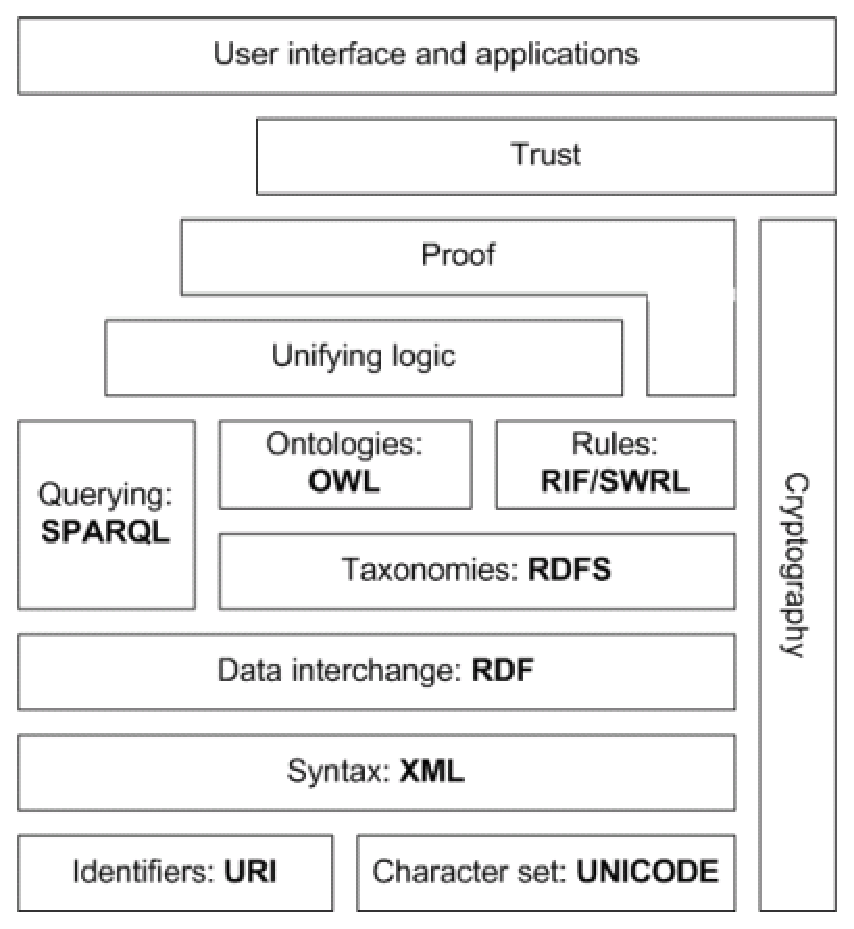
\includegraphics[height=\textheight]{../pics/semantic-web-layers.eps}

\myslide{Identifiers and Characters}

\begin{itemize}
\item Characters are always defined using Unicode
\item Identifiers are \blu{Uniform Resource Identifiers}
  \begin{itemize}
  \item \blu{Universal Resource Name}
    \begin{itemize}
    \item e.g., \url{urn:isbn:1575864606}
    \item uniquely identifies one edition of a book
    \end{itemize}
  \item \blu{Universal Resource Locator:}
    \begin{itemize}
    \item \texttt{scheme:part?query\#anchor}
    \item e.g., \url{http://www3.ntu.edu.sg/home/fcbond/}
    \item http, skype, ssh, secondlife, \ldots
    \end{itemize}
  \end{itemize}
\item Identifies or names a resource on the web
\end{itemize}


\myslide{XML: eXtensible Markup Language}

\begin{itemize}
\item XML is a set of rules for encoding documents electronically.
\item Based on a simplified SGML
\item XML’s design goals emphasize simplicity, generality, and usability.
\item It is a textual data format
\item It supports many encodings, with Unicode preferred
\item It can represent arbitrary data structures, for example in web services.
\end{itemize}

\myslide{In other words}

\begin{itemize}
\item \blu{XML} stands for \blu{EXtensible Markup Language}
\item is a markup language much like HTML
\item was designed to \blu{carry data, not to display data}
\item tags are not predefined. You must define your own tags
\item is designed to be \blu{self-descriptive}
\item XML is a W3C Recommendation
\end{itemize}

%%% FIXME how different from text?

\myslide{With XML You Invent Your Own Tags}

\begin{verbatim}
<bitext> 
<author xml:lang="eng">Francis Bond</author> 
<author xml:lang="jpn">フランシス ボンド</author>
<email>fcbond@ntu.edu.sg</email> 
<opendata>yes</opendata>
\end{verbatim}

\begin{itemize}
\item The tags describe the content, but do not do anything.
\item You have to define the meaning elsewhere
\end{itemize}

\myslide{XML structure}

\begin{itemize}
\item An \blu{XML element} looks like this
\\ \texttt{<tag attribute='value'>Content</tag>}
  \begin{itemize}
\item You can use \blu{attributes} (easy to verify)
\begin{verbatim}
<author xml:lang="eng">Francis Bond</author>
\end{verbatim}
  \item or \blu{nested elements} (flexible)
\begin{verbatim}
<author>
  <lang>eng</lang>
  <name>Francis Bond</name>
</author>
\end{verbatim}
  \end{itemize}
\item If all elements are written correctly the document is 
\emp{well formed}
\end{itemize}


\myslide{XML with structure highlighted}

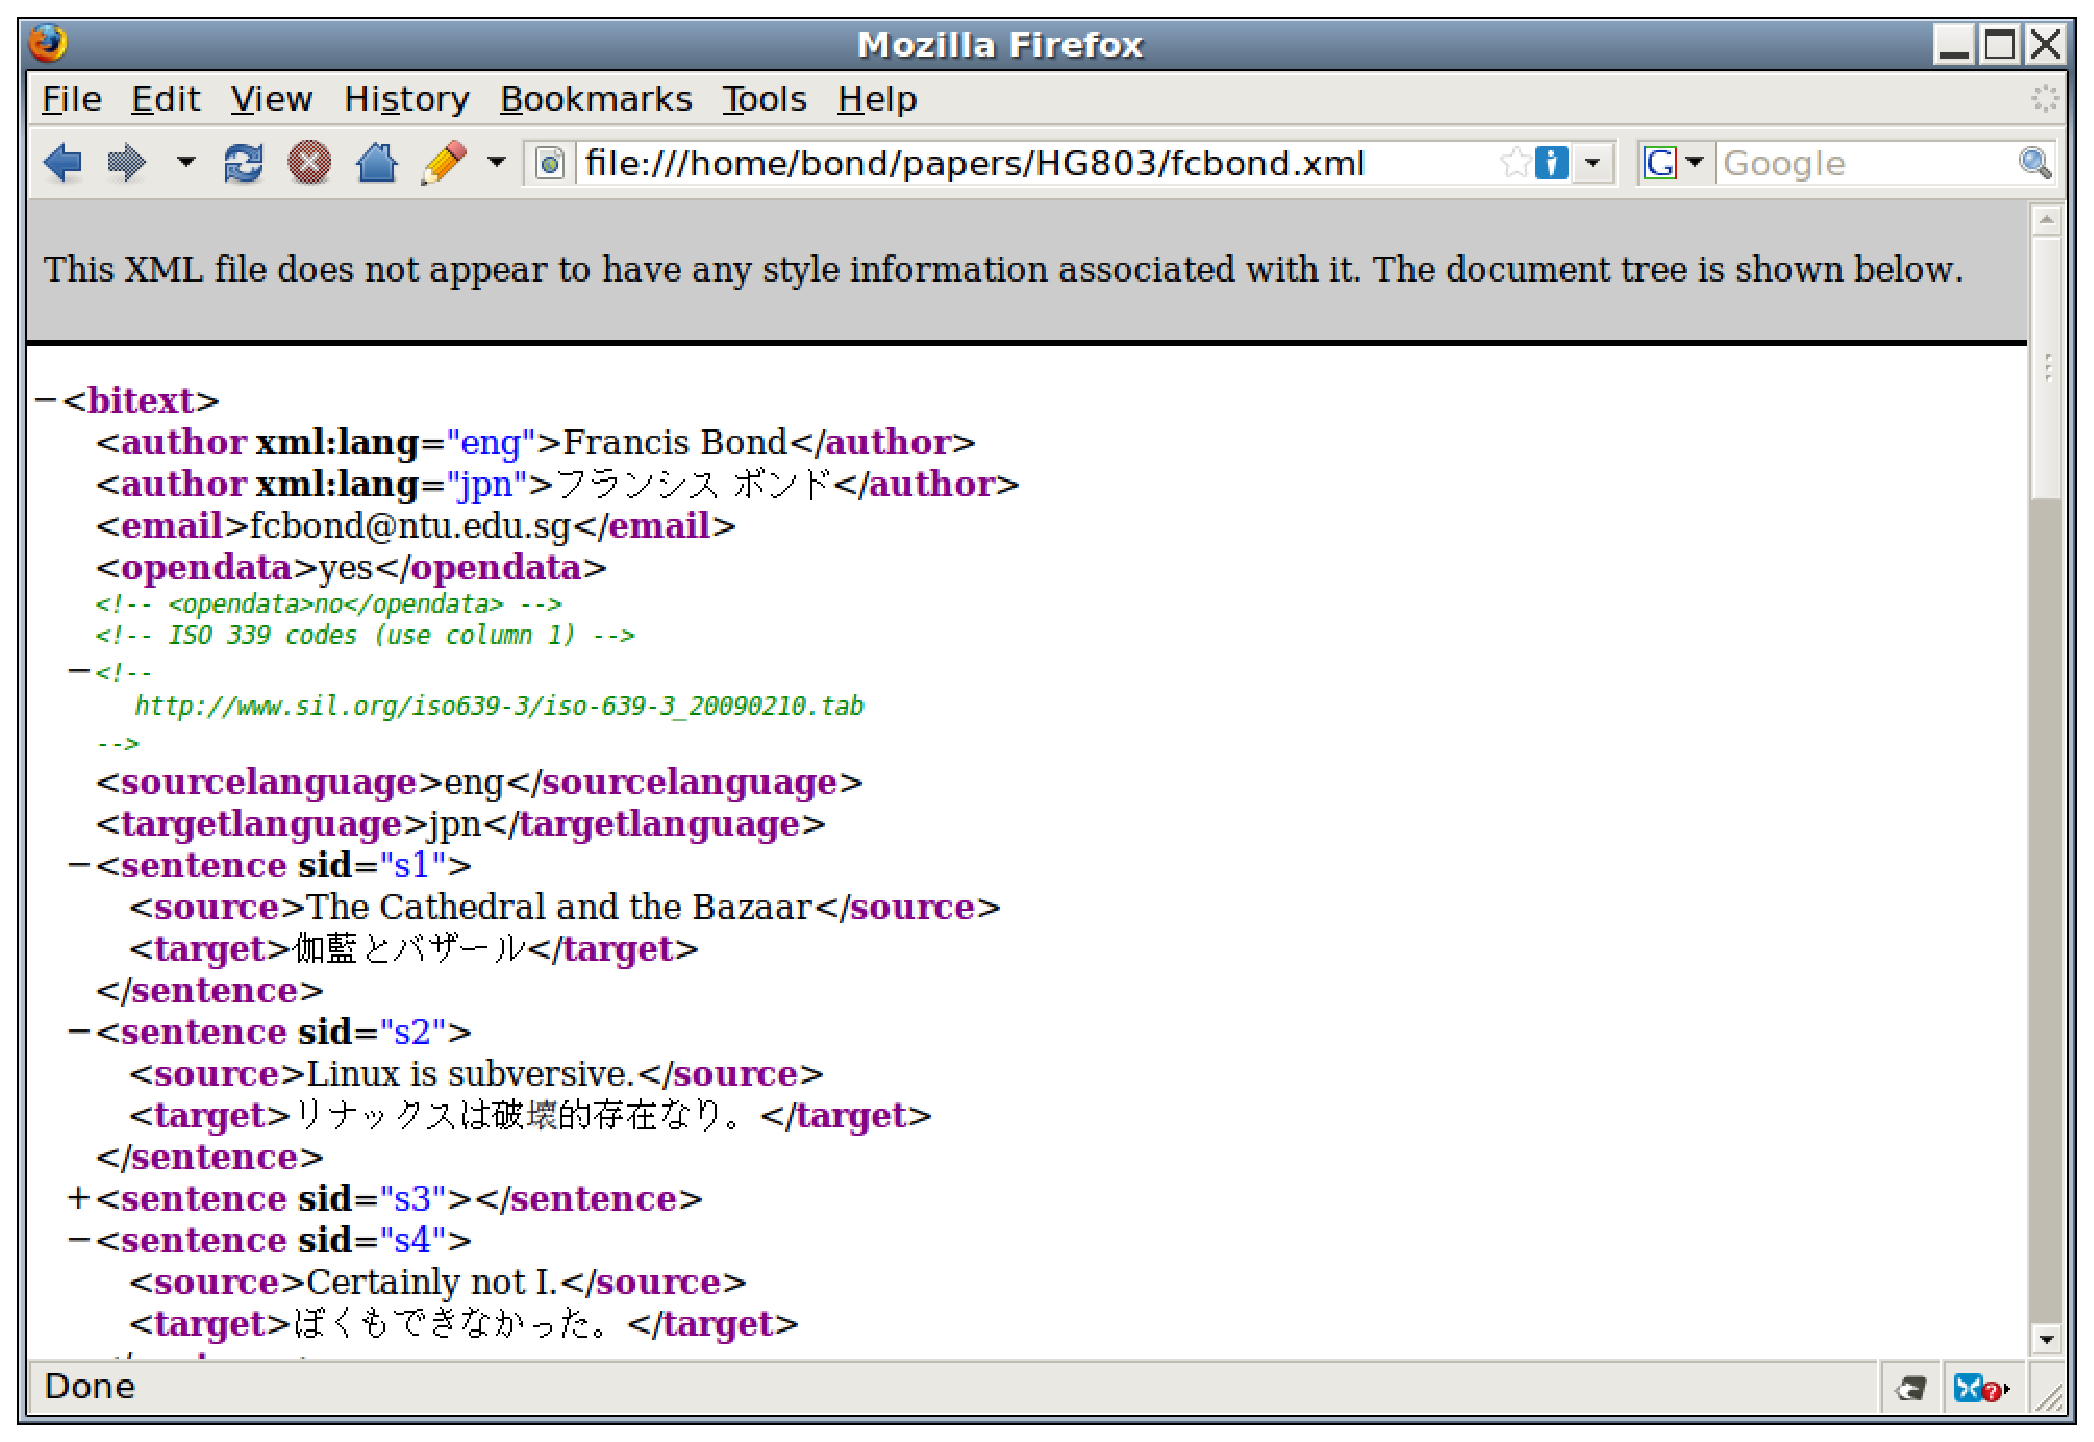
\includegraphics[height=\textheight]{../pics/xml-sample.eps}

\myslide{Document Type Definitions}

\begin{itemize}
\item You can also define what tags are possible with 
  \begin{itemize}
  \item DTD (\blu{Document Type Definition})
  \item XML Schema
  \end{itemize}
\begin{verbatim}
<!DOCTYPE bitext
[
<!ELEMENT author (#PCDATA)>
<!ATTLIST author xml:lang CDATA>
<!ELEMENT sentence (source,target)>
...
\end{verbatim}
\item This makes the structure explicit
\end{itemize}

\myslide{Why Use a DTD?}
\begin{itemize}
\item With a DTD, XML files \blu{can carry a description of their own format}.
\item With a DTD, independent groups of people can use a well defined, enforceable standard  for interchanging data.
\item Your application can use a standard DTD to verify that the data you receive from the outside world is valid.
\item You can also use a DTD to verify your own data.
  \begin{itemize}
  \item \emp{You can catch format errors early}
  \end{itemize}
\item \textbf{BUT}, XML only defines \blu{structure} not \blu{content}
\end{itemize}

\myslide{Validation}

\begin{itemize}
\item Validation is very important
\item Ill-formed data makes parsing complex
\item Early detection of errors is cost-effective
\item Validated data is easy to maintain
\end{itemize}

\myslide{Semantic Web Architecture}

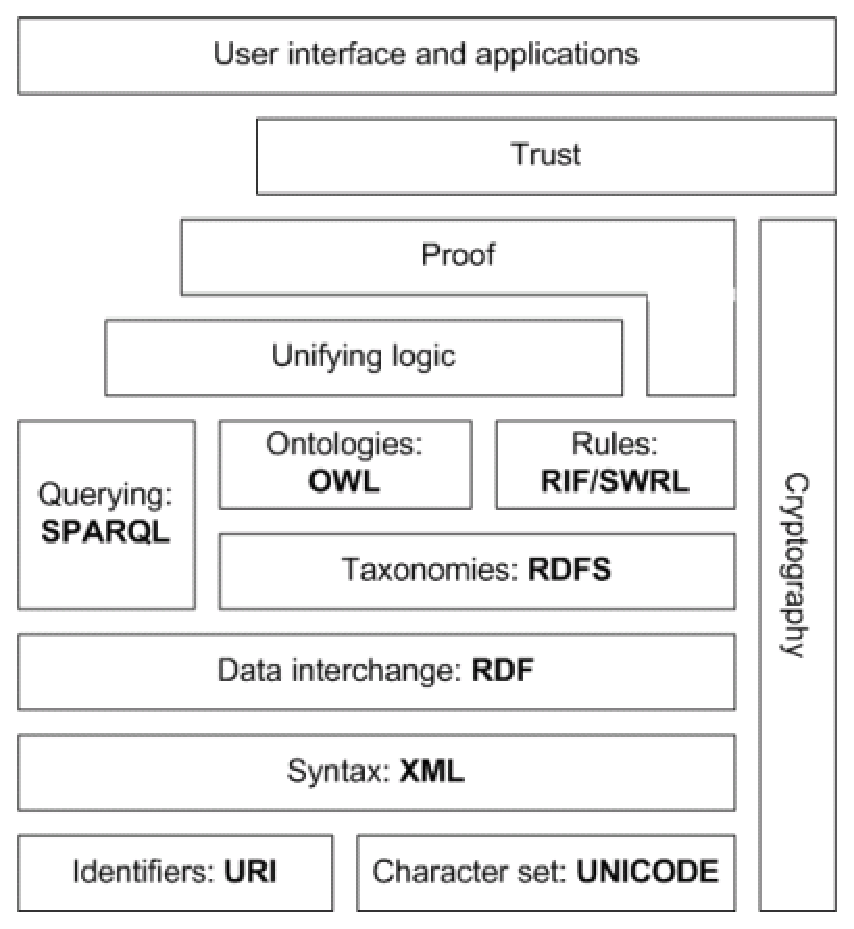
\includegraphics[height=\textheight]{../pics/semantic-web-layers.eps}

\myslide{RDF: Resource Description Framework}

\begin{itemize}
\item We want to identify content
\item Annotate information with descriptions:
  \\ \blu{triples of information}
  \begin{itemize}
  \item subject 
  \item \iz{predicate}
  \item object
  \end{itemize}
 e.g. $<$dog, \iz{hyponym}, animal$>$ 
\\ e.g. $<$Francis Bond, \iz{teacher}, HG252$>$
\item The trick is that each element is a \emp{URI}
\item You can say anything about anything
\end{itemize}

\myslide{RDF graph describing Eric Miller}


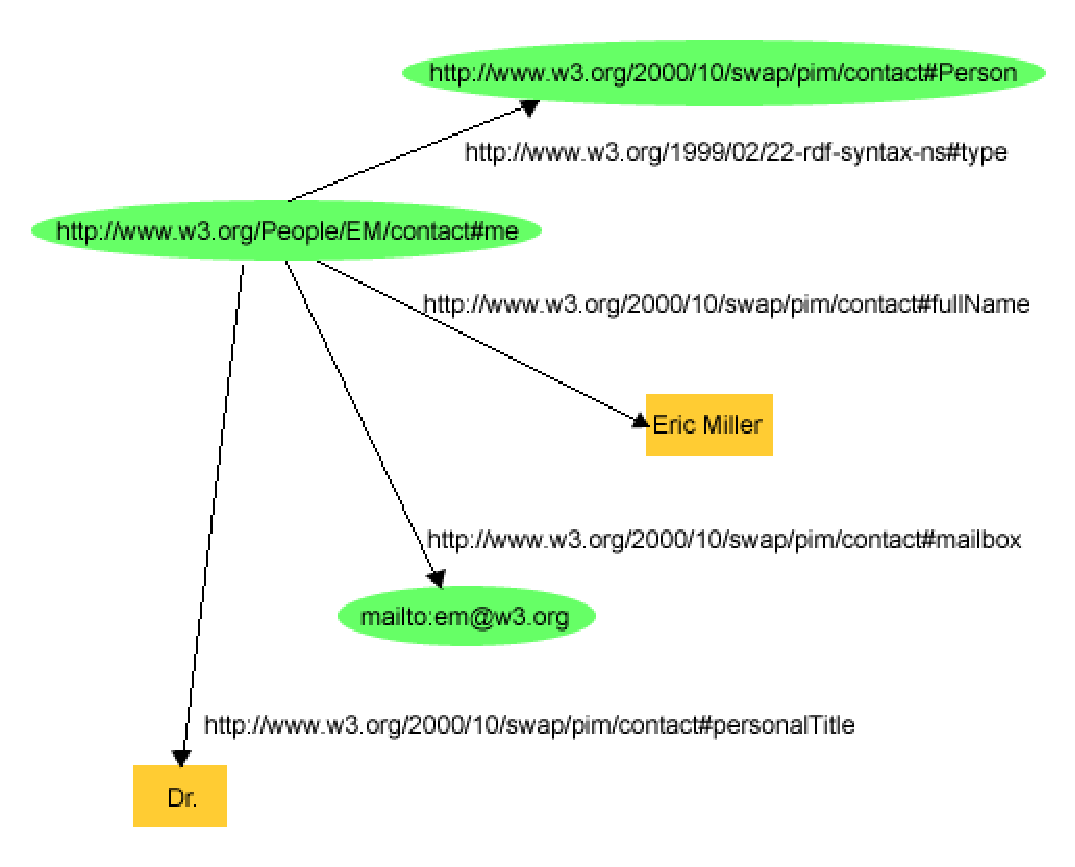
\includegraphics[height=0.8\textheight]{../pics/miller-rdf.eps}

Relational Semantic Representation (again!), 
\\ with relations defined by URIs

\myslide{RDFs are written using XML}

\begin{small}
\begin{verbatim}
<?xml version="1.0"?>
<rdf:RDF xmlns:rdf="http://www.w3.org/1999/02/22-rdf-syntax-ns#"
         xmlns:contact="http://www.w3.org/2000/10/swap/pim/contact#">

  <contact:Person rdf:about="http://www.w3.org/People/EM/contact#me">
    <contact:fullName>Eric Miller</contact:fullName>
    <contact:mailbox rdf:resource="mailto:em@w3.org"/>
    <contact:personalTitle>Dr.</contact:personalTitle> 
  </contact:Person>

</rdf:RDF>
\end{verbatim}
\end{small}
\begin{itemize}
\item Not designed for people to read (or write) directly
\item Designed to be extensible and explicit
\end{itemize}

\myslide{Why use URIs in RDFs with XML?}

\begin{itemize}
\item A shared URI gives a shared definition 
\item You can add new URIs as necessary
\item RDFs are complicated
  \begin{itemize}
  \item you need to validate the syntax \into XML
  \end{itemize}
\item RDFs assume the existence of the web
  \begin{itemize}
  \item Nothing has meaning on its own
  \item \textit{You shall know a URI by the company it keeps}
  \end{itemize}
\end{itemize}

\myslide{OWL and Ontologies}

\begin{itemize}
\item Allowing any URI makes information hard to combine
\item Use Ontologies to link it together again
  \begin{itemize}
  \item You can normally agree on a hypernym (supertype)
  \end{itemize}
\item Agreeing on an ontology is difficult
  \begin{itemize}
  \item Many detailed ontologies
  \item One common ontology
    \begin{itemize}
    \item The Standard Upper Merged Ontology (SUMO)
    \item Links many ontologies (including WordNet)
    \end{itemize}
  \item Much recent work on medical and library domains
  \end{itemize}
\end{itemize}

\myslide{Common Semantic Web Ontologies}

\begin{itemize}
\item People + Organisations
  \begin{itemize}
  \item FOAF, HCard, Relationship, Resume 
  \end{itemize}
\item Places
  \begin{itemize}
  \item Geonames, Geo 
  \end{itemize}
\item Events
  \begin{itemize}
  \item RDFCalendar 
  \end{itemize}
\item Social Media
  \begin{itemize}
  \item SIOC, Review 
  \end{itemize}
\item Topics + Tags
  \begin{itemize}
  \item SKOS, MOAT, HolyGoat 
  \end{itemize}
\item eCommerce
  \begin{itemize}
  \item GoodRelations, CC Licensing 
  \end{itemize}
\item More...
  \begin{itemize}
  \item Scovo, DOAP, Recipes, Measurements, ... 
  \end{itemize}
\item General things
  \begin{itemize}
  \item SUMO, WordNet
  \end{itemize}
\end{itemize}



\myslide{Semantic Web Architecture}

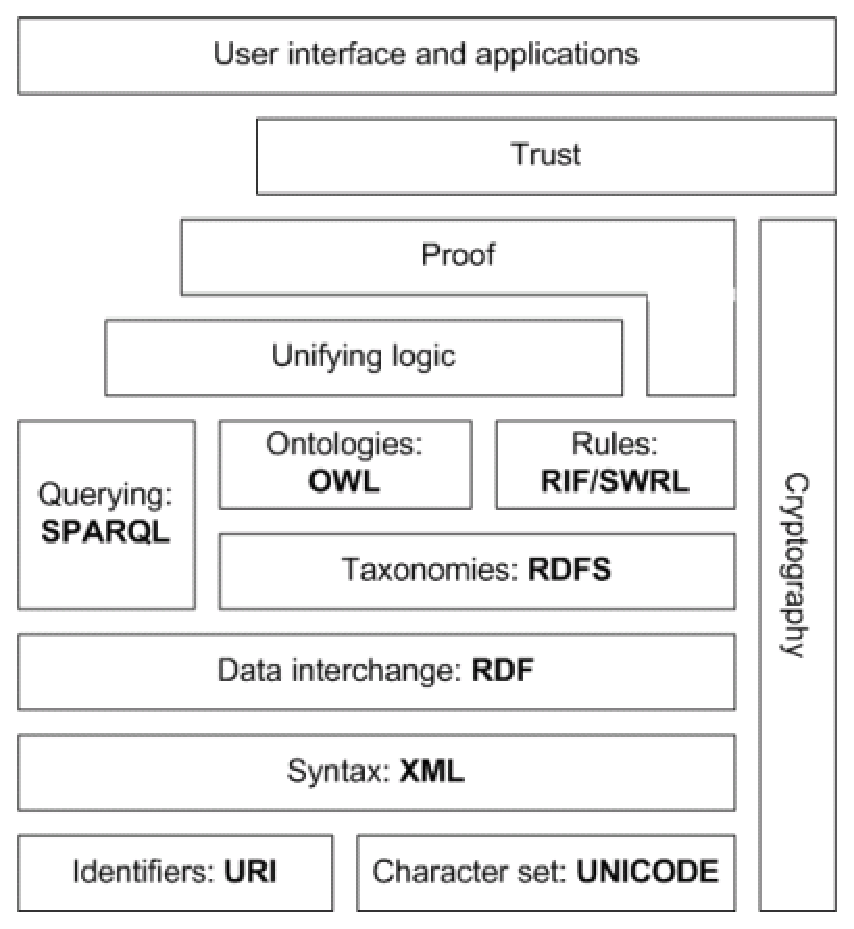
\includegraphics[height=\textheight]{../pics/semantic-web-layers.eps}

\myslide{The upper layers}

\begin{itemize}
\item Querying the (semantic) web is 
  \begin{itemize}
  \item Slow (non local access \into millions of times slower)
  \item Non-deterministic (the answers change)
  \item Vast (could be trillions of elements)
  \end{itemize}
  A whole new set of technical problems
\item Logic, Proof and Trust are still works in progress
  \begin{itemize}
  \item Reusing AI research from the 70s and 80s
  \end{itemize}
\item But applications are going along without them
  \begin{itemize}
  \item Enhanced search using metadata
  \item Combinations of data
  \end{itemize}
\end{itemize}


\myslide{Semantic Web Lessons}

\begin{itemize}
\item RDF as a general information model is applicable to many uses 
\\ (many of which we never even thought about)
\item Common data representation and architecture drives down costs
\\  (technical and social)
\item Facilitates serendipitous interoperability 
\\ - breaking down the barriers of domain knowledge
\item When "Anyone can say anything about anything", 
\\ who you trust is important (same as in text mining)

\item Beneficial to solving interoperability in Open (rather than Closed) systems

\end{itemize}

 
\myslide{Summary}

\begin{itemize}
\item The goal of the Semantic Web is to share knowledge
  \begin{itemize}
  \item Uses markup to give tractable annotation
    \begin{itemize}
    \item Unicode
    \item XML
    \item URI
    \item RDF
    \item OWL
    \end{itemize}
  \item Relies on web resources to make common assumptions explicit
\end{itemize}
\end{itemize}

\myslide{Example of making information explicit}

\begin{center}
  $<$ Francis Bond, author, Translating the Untranslatable $>$
\end{center}

\begin{itemize}
    \item Francis Bond: \url{http://www3.ntu.edu.sg/home/fcbond/}
      \begin{itemize}
      \item defined using Francis Bond's homepage 
      \end{itemize}
    \item author: \url{http://purl.org/dc/elements/1.1/creator} 
      \begin{itemize}
      \item  defined using the Dublin Core Ontology 
      \end{itemize}
  \item[or] \url{http://nlpwww.nict.go.jp/wn-synset.cgi?synset=10794014-n}
  \begin{itemize}
      \item  defined using WordNet
      \end{itemize}
    \item  Translating the Untranslatable: \url{urn:isbn:1575864606}
      \begin{itemize}
      \item  defined using the ISBN ontology
      \end{itemize}

  \end{itemize}

\myslide{An Example of Data Integration}

\begin{itemize}
\item Map the various data onto an abstract data representation
 \begin{itemize}
\item  make the data independent of its internal representation
\end{itemize}
\item Merge the resulting representations
\item Start making queries on the whole!
 \begin{itemize}
\item queries that could not have been done on the individual data sets
\end{itemize}
\end{itemize}

\begin{flushright}
  Slides from ``An introduction to the Semantic Web (Through an Example)'' 
  \\ By Ivan Herman (\url{http://www.w3.org/People/Ivan/CorePresentations/IntroThroughExample/})
\end{flushright}

\myslide{A simplified bookstore data (dataset ``A'')}

\noindent
\begin{itemize}\addtolength{\itemsep}{-1ex}

\item Book
  \begin{itemize}
  \item ID: 000651409X
  \item Author: A11
  \item Title: The Glass Palace
  \item Publisher: P202
  \item Year: 2000
  \end{itemize}
\item Person:
  \begin{itemize}
  \item ID: A11 
  \item Name: Amitav Ghosh
  \item Homepage: www.amitavghosh.com
  \end{itemize}
\item Publisher:
  \begin{itemize}
  \item ID: P202 
  \item Name: Harper Collins
  \item Address: London
  \end{itemize}

\end{itemize}
% 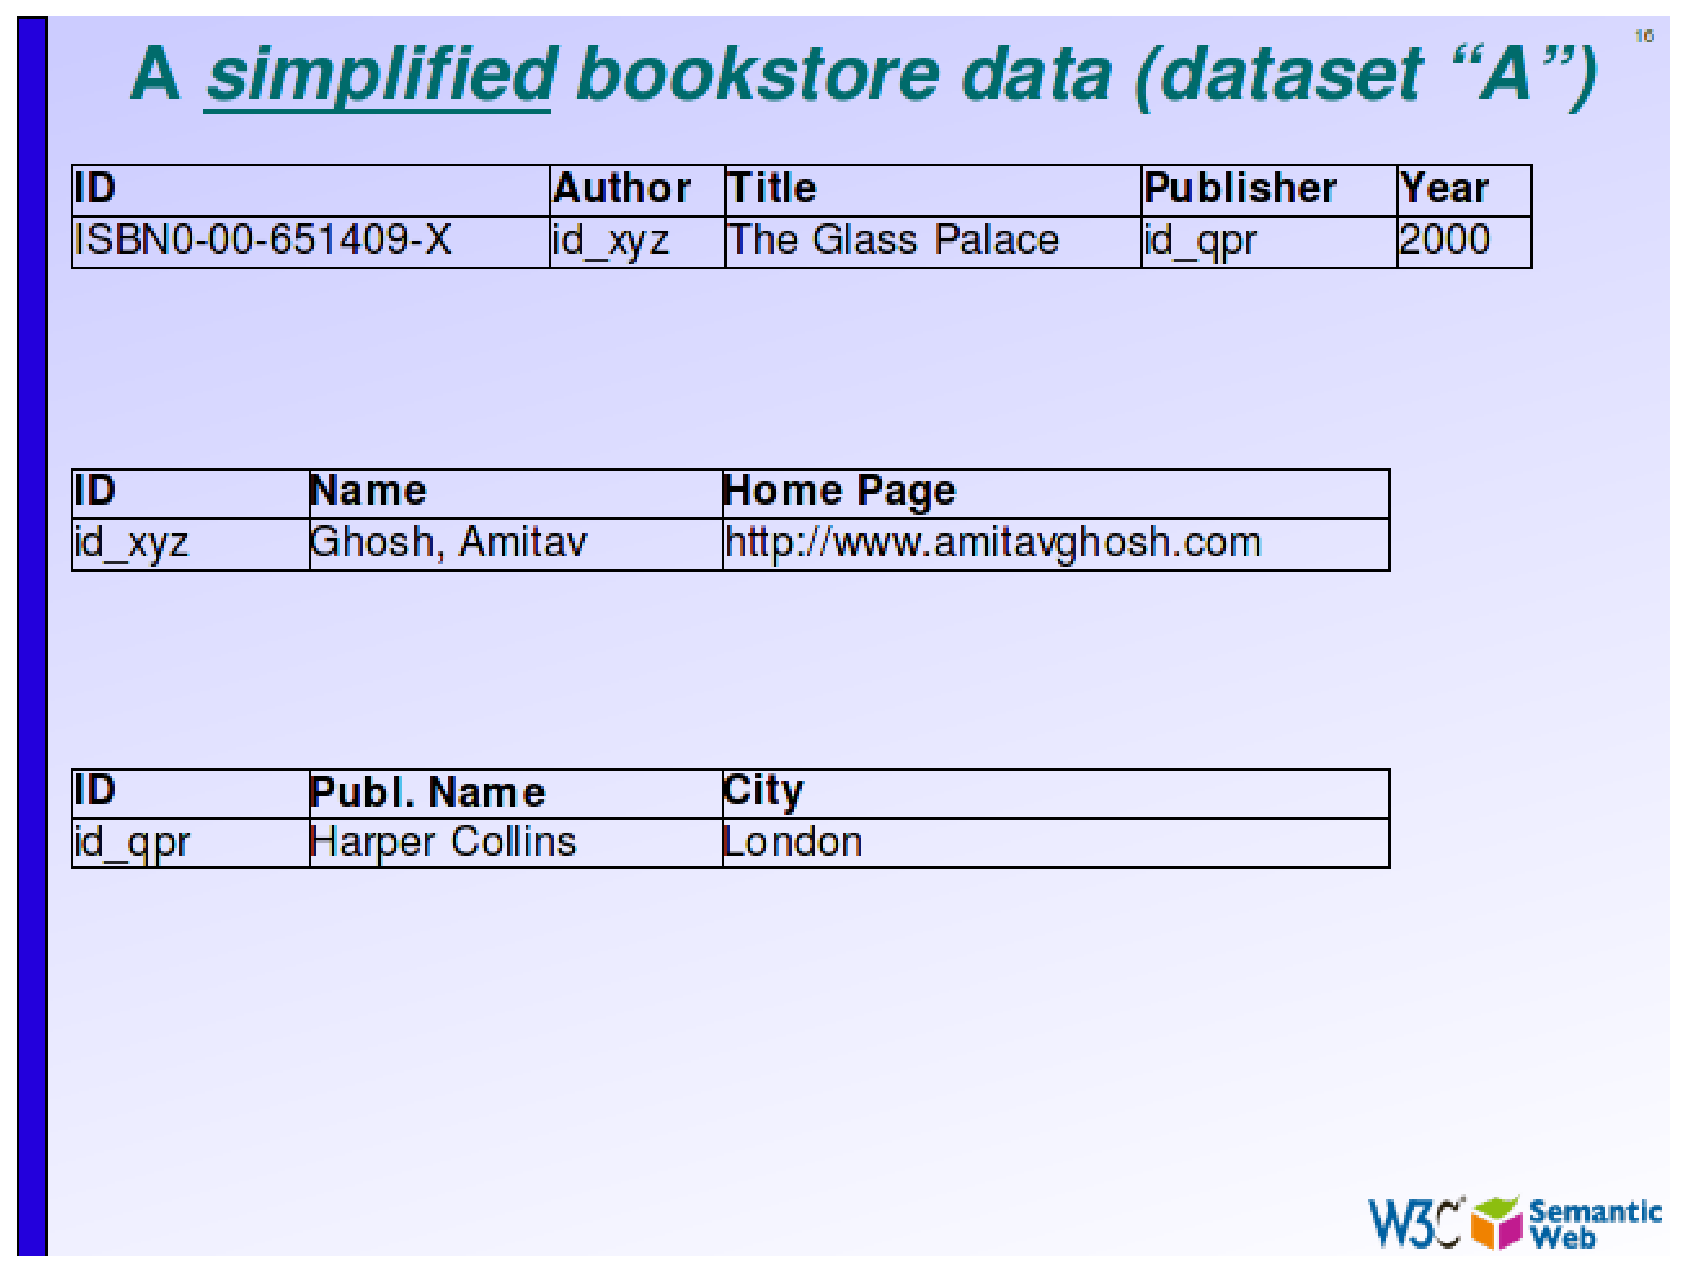
\includegraphics[trim= 0mm 35mm 0mm 20mm, clip=true, 
%                  width=\textwidth]{../pics/img15.png.eps}

\myslide{Export your data as a set of relations}

\noindent
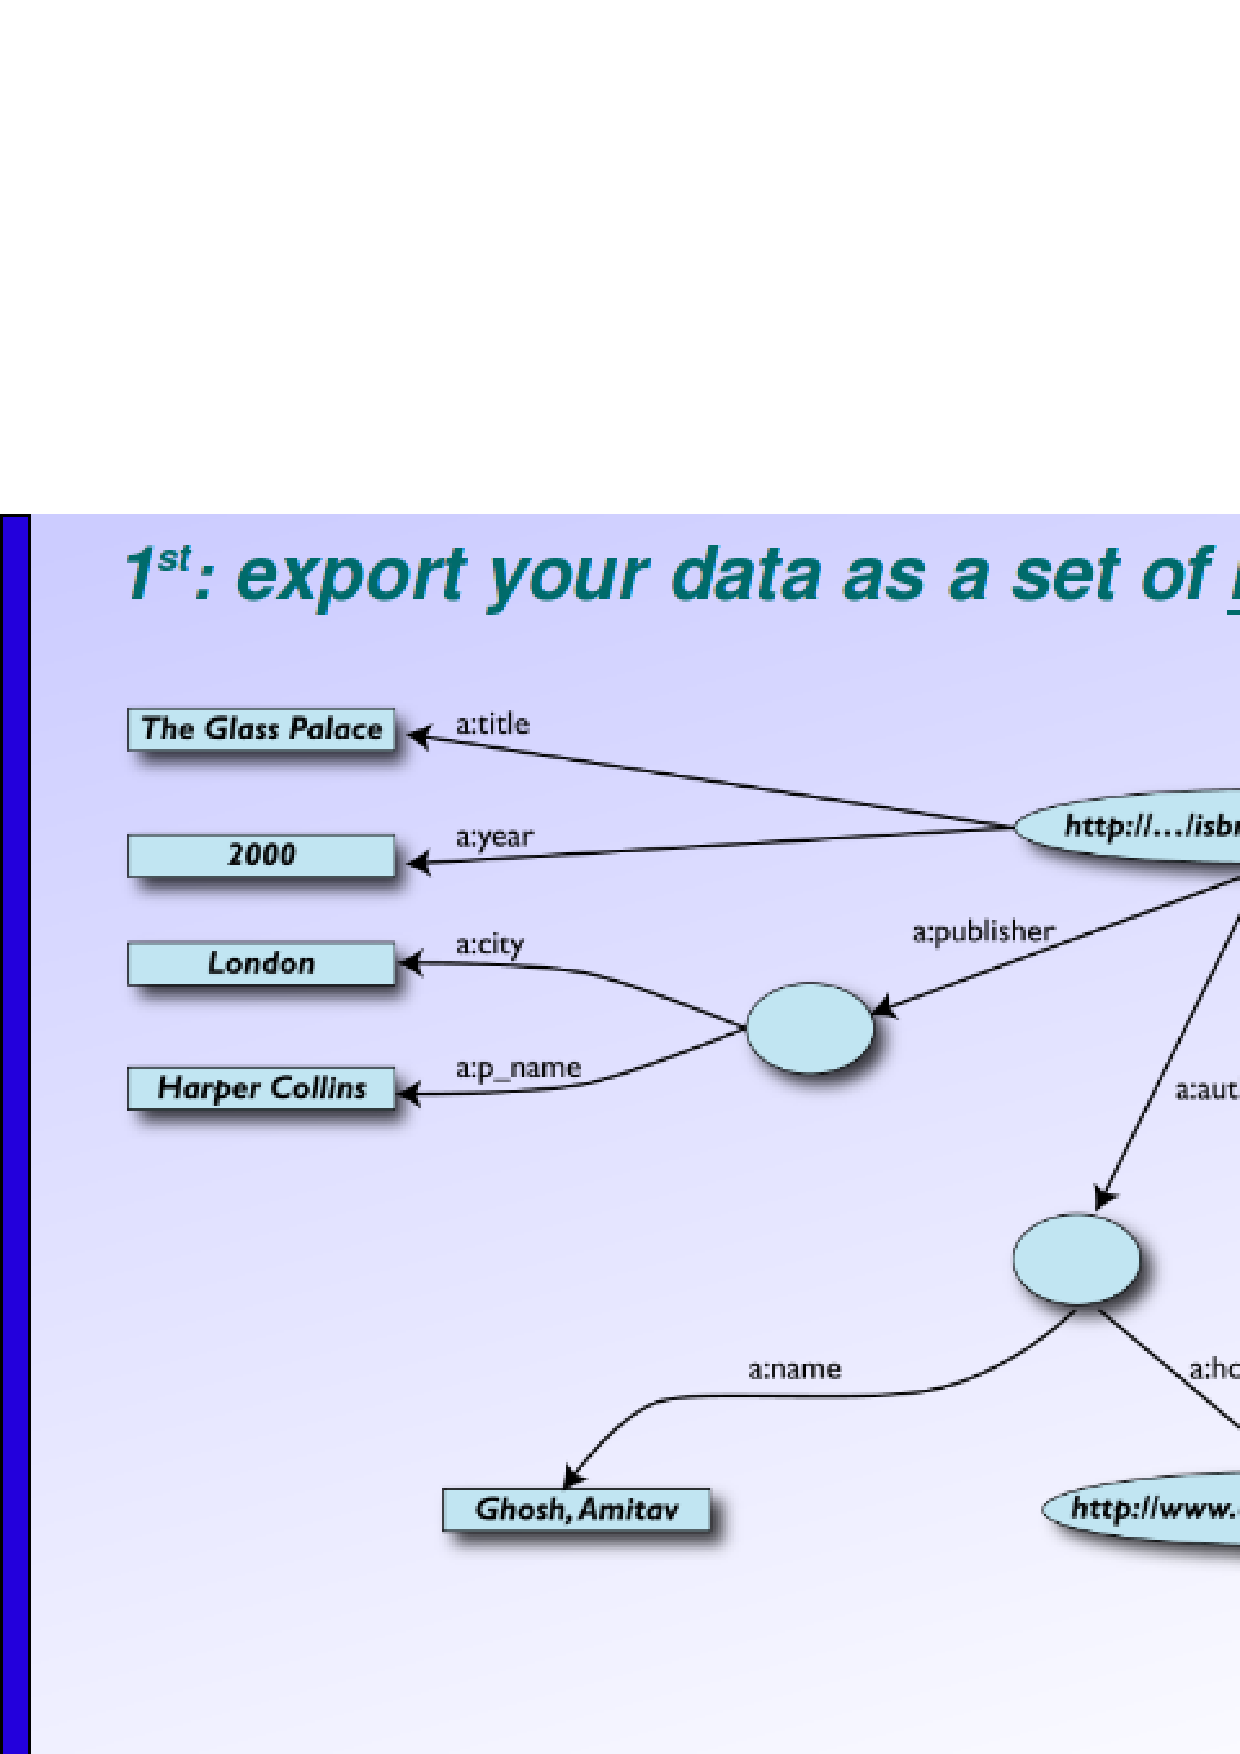
\includegraphics[width=\textwidth]{../pics/img16.png}


\myslide{Some notes on the exporting the data}

\begin{itemize}
\item Relations form a graph
  \begin{itemize}
  \item the nodes refer to the ``real'' data or contain a string
  \item how the graph is represented in machine is immaterial for now
  \item Data export does not necessarily mean physical conversion of the data
    \begin{itemize}
    \item relations can be generated on-the-fly at query time
      \begin{itemize}
      \item via SQL ``bridges''
      \item scraping HTML pages
      \item extracting data from Excel sheets
      \item through text mining
      \item etc.
      \end{itemize}
    \item One can export part of the data
    \end{itemize}
  \end{itemize}
\end{itemize}

\myslide{Another Set of Data (set ``F'')}

%\noindent
%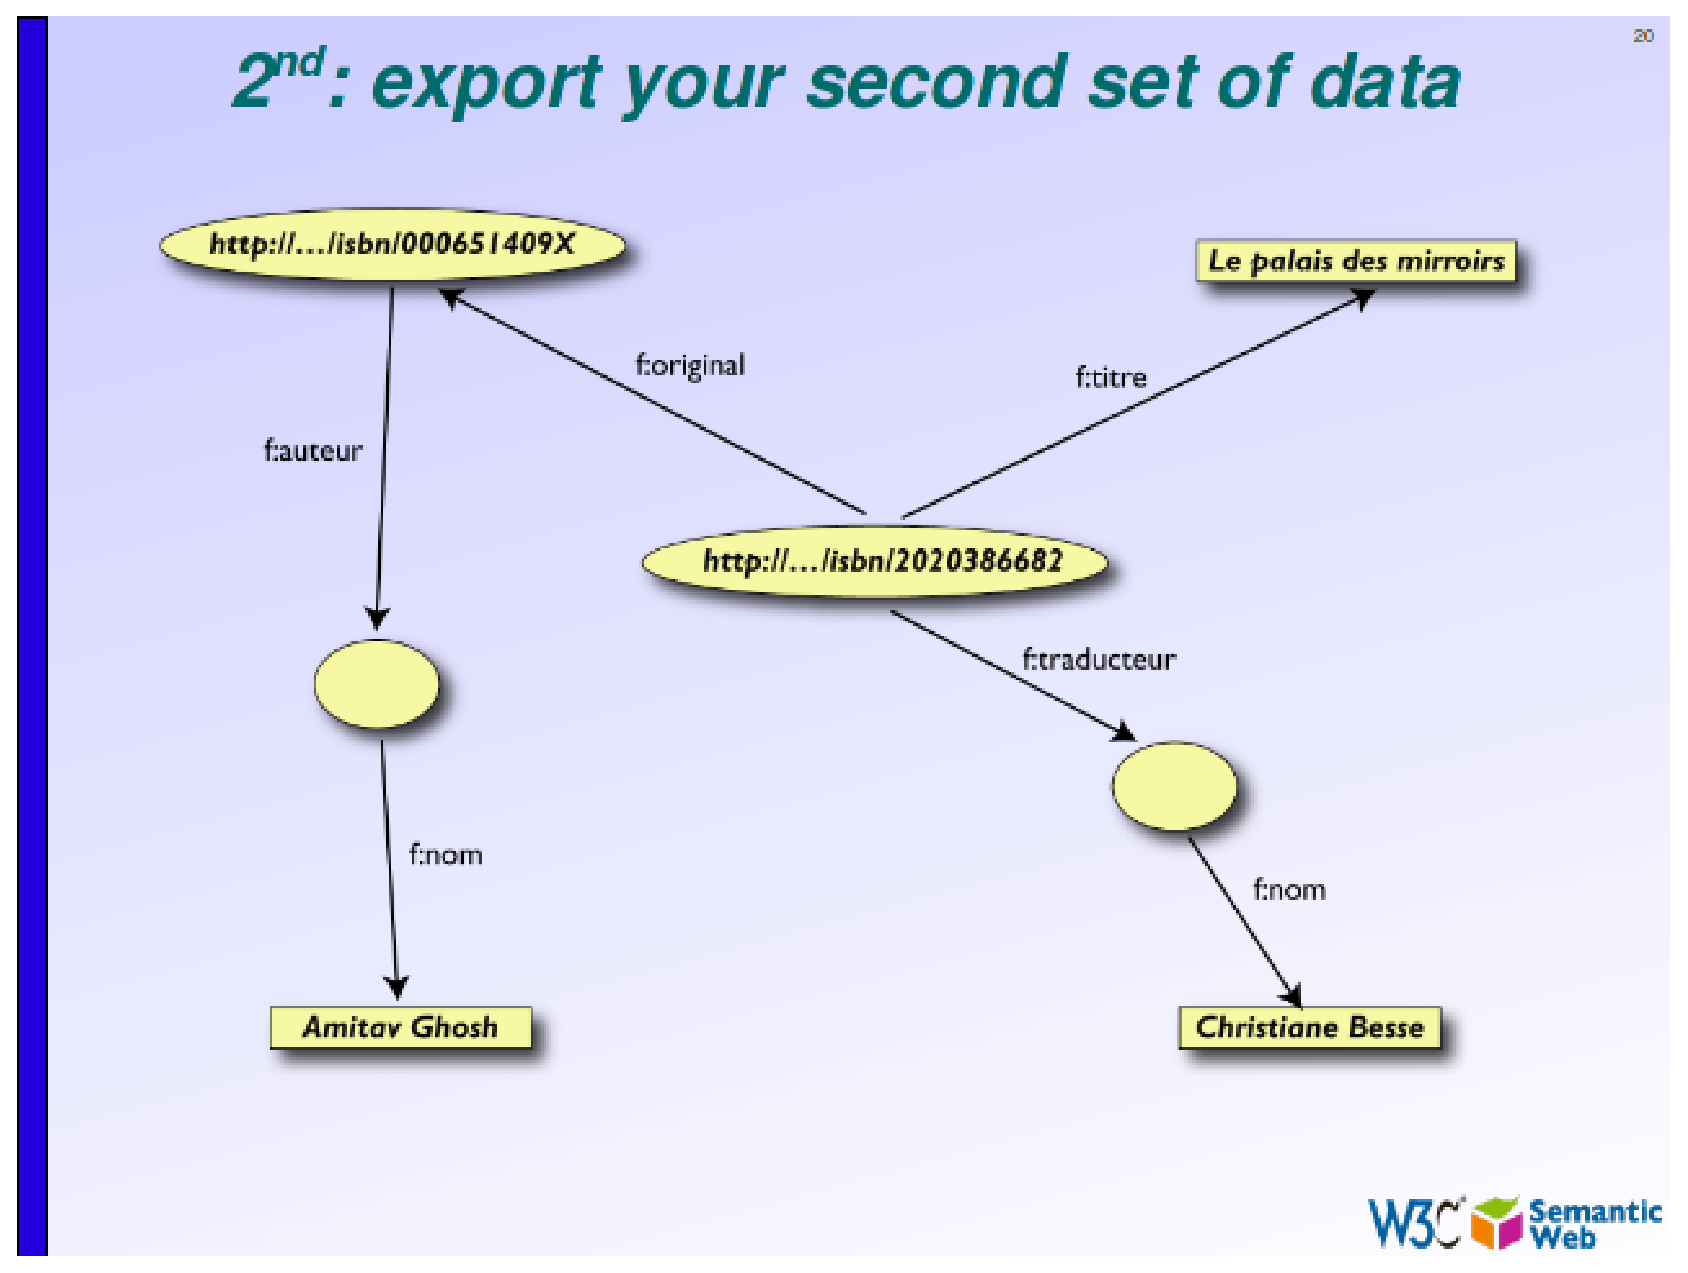
\includegraphics[width=\textwidth]{../pics/img19.png.eps}

\begin{itemize}\addtolength{\itemsep}{-1ex}
\item Book
  \begin{itemize}
  \item ID: ISBN 20203866682
  \item Titre: la Palais des miroirs
  \item Traducteur: P2
  \item Original: ISBN 000651409X
  \end{itemize}
\item Book
  \begin{itemize}
  \item ID: 000651409X
  \item Auteur: P1
  \end{itemize}
\item Person:
  \begin{itemize}
  \item ID: P1 
  \item Nom: Ghosh, Amitav
  \end{itemize}
\item Person:
  \begin{itemize}
  \item ID: P2 
  \item Nom: Besse, Christianne
  \end{itemize}

\end{itemize}


\myslide{Export Set F}

\noindent
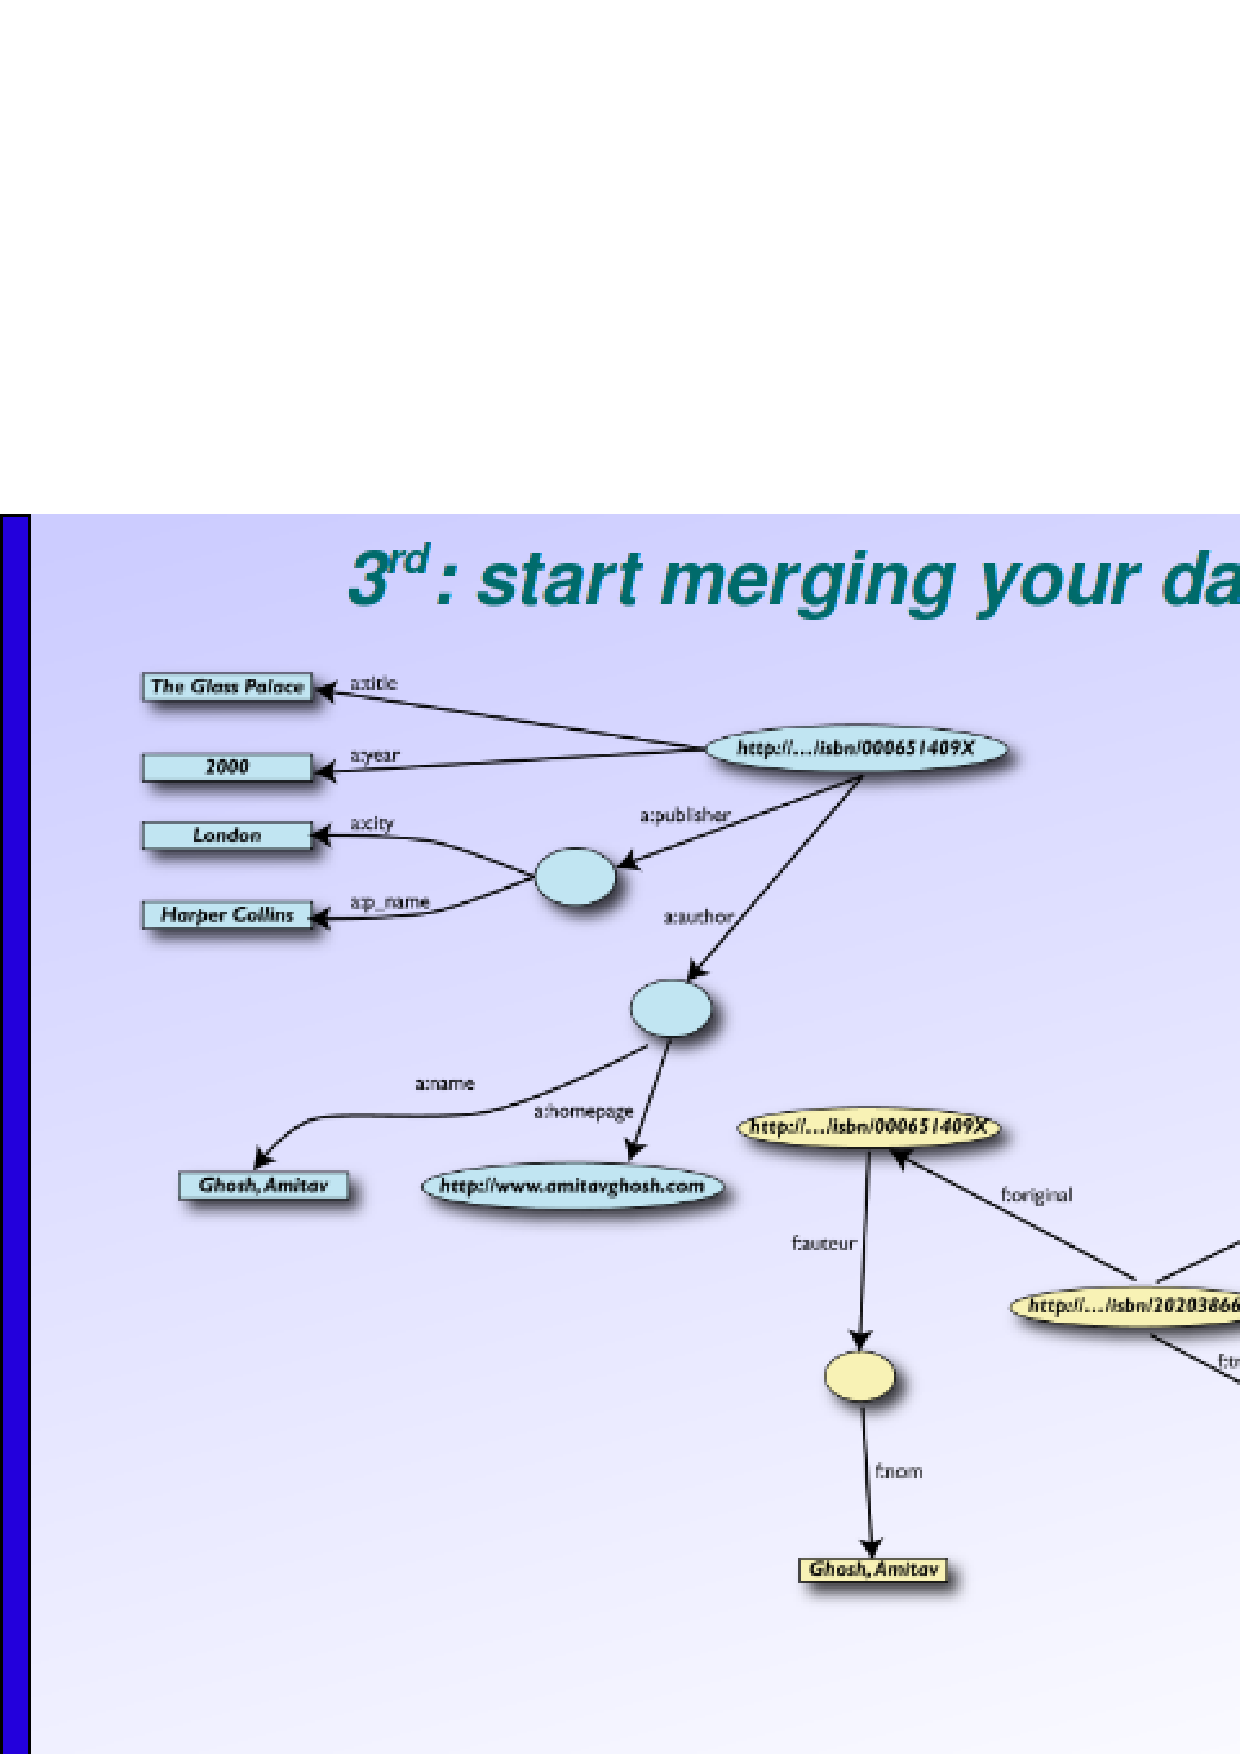
\includegraphics[width=\textwidth]{../pics/img20.png}

\myslide{Start to Merge}

\noindent
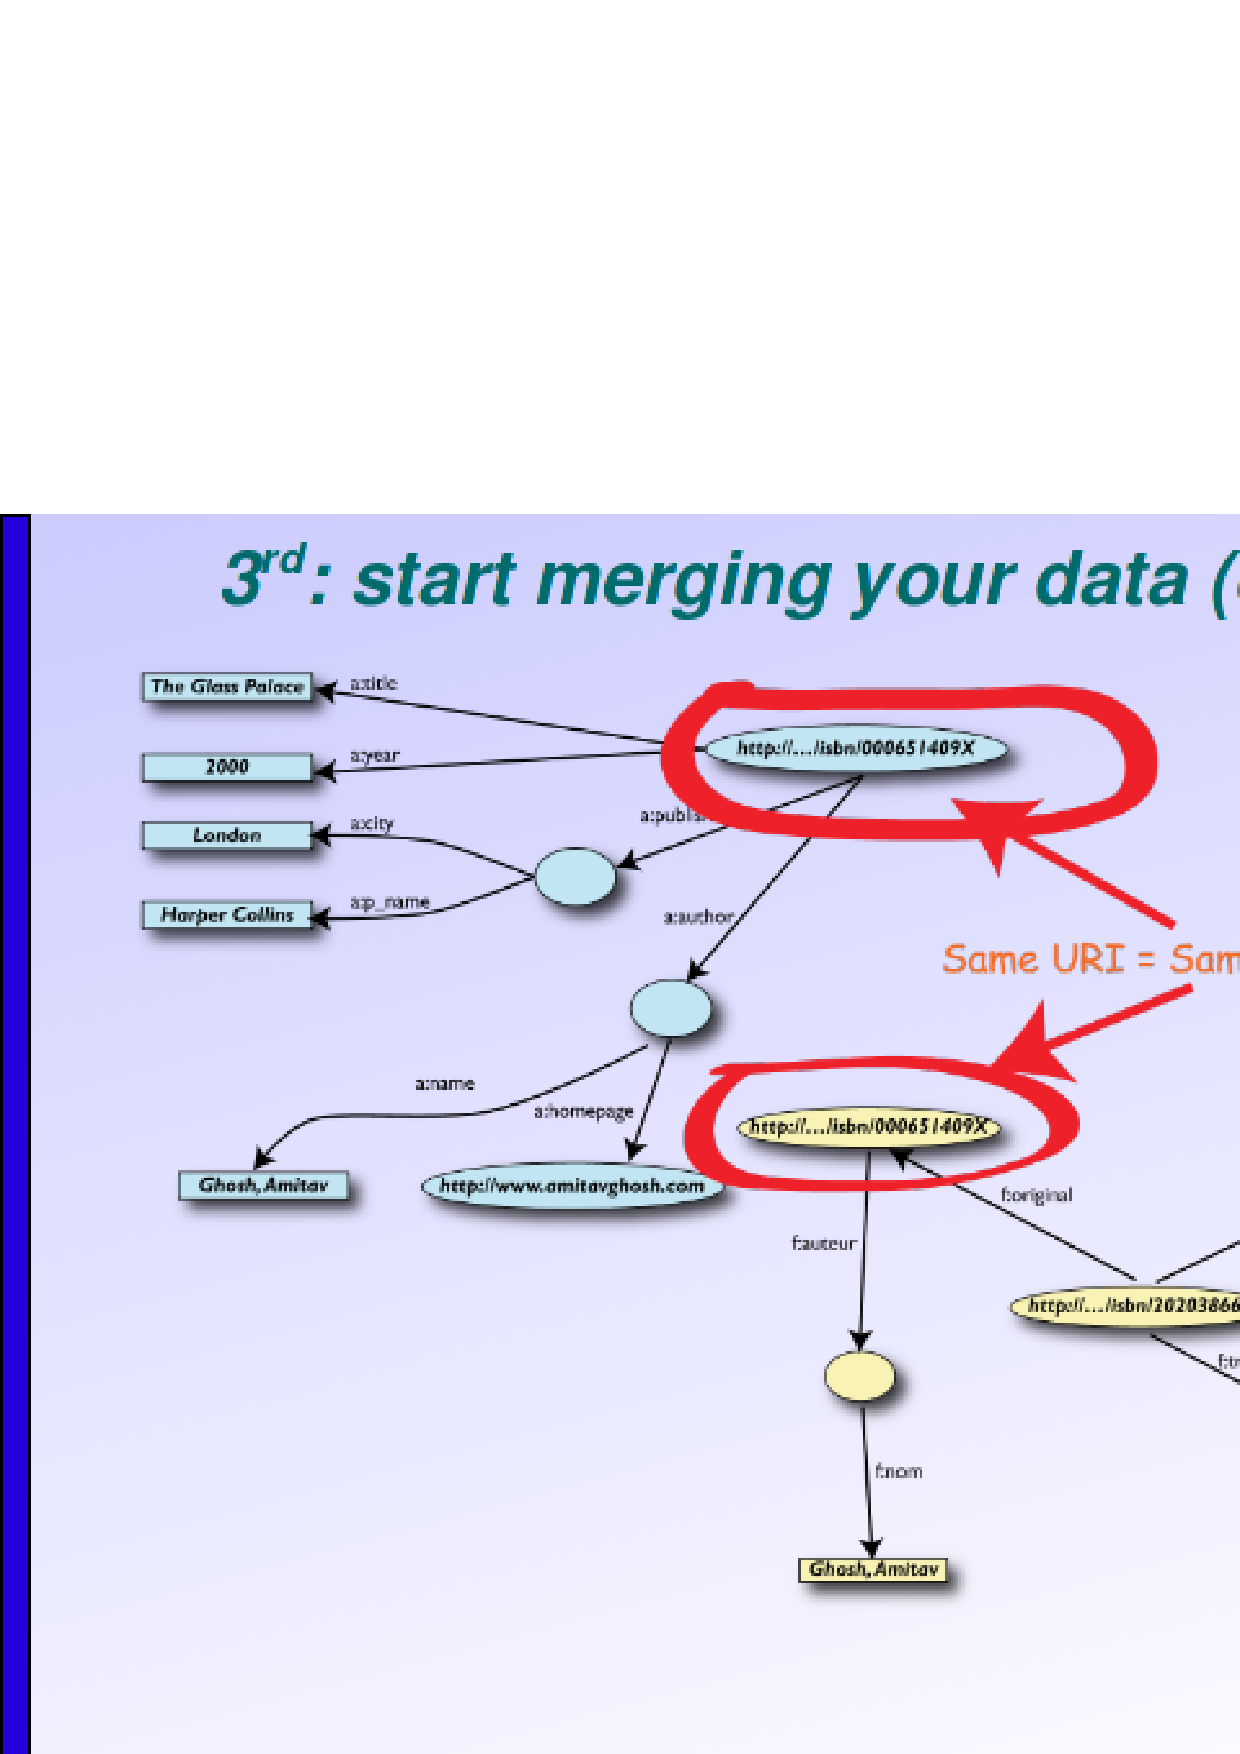
\includegraphics[width=0.9\textwidth]{../pics/img21.png}

\myslide{Merge Identical Resources}

\noindent
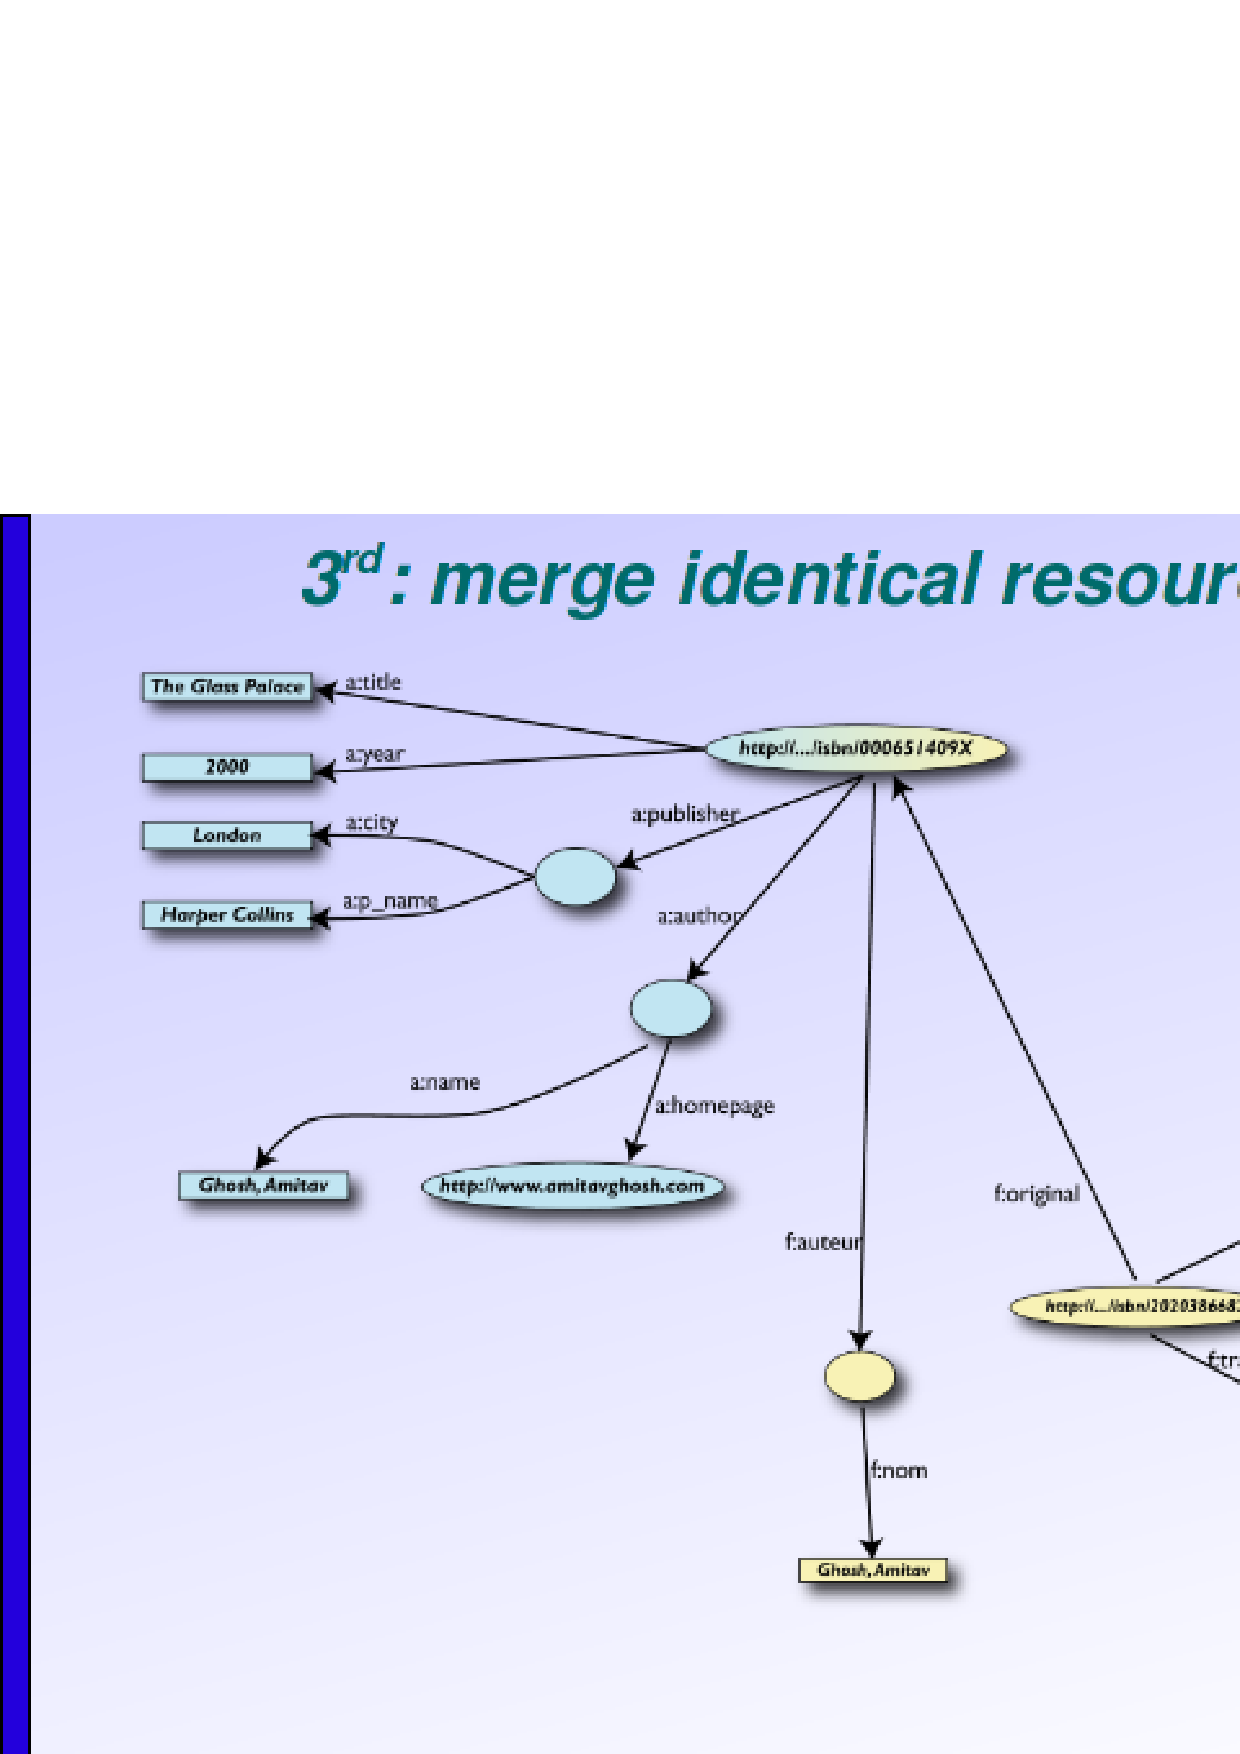
\includegraphics[width=0.9\textwidth]{../pics/img22.png}

% \myslide{

% \noindent
% \includegraphics[trim= 0mm 35mm 0mm 20mm, clip=true, 
%                  width=\textwidth]{../pics/img23.png.eps}


\myslide{Start making queries}

\begin{itemize}
\item User of data ``F'' can now ask queries like:
  \begin{itemize}
  \item ``give me the title of the original''
  \item  well, ``donnes-moi le titre de l’original''
  \end{itemize}
\item This information is not in the dataset ``F''
\item \ldots but can be retrieved by merging with dataset ``A''!
\end{itemize}


\myslide{However, more can be achieved}

\begin{itemize}
\item We ``feel'' that \blu{a:author} and \blu{f:auteur} should be the same
\item But an automatic merge doest not know that!
  \begin{itemize}
  \item If only we could understand language
  \item They both point to the same synset in wordnet (or at least one)
  \end{itemize}
\item Let us add some extra information to the merged data:
  \begin{itemize}
  \item \blu{a:author} same as \blu{f:auteur}
  \item both identify a ``Person''
  \item a term that a community may have already defined:
    \begin{itemize}
    \item a ``Person'' is uniquely identified by his/her name and, say, homepage
    \item it can be used as a ``category'' for certain type of resources
    \end{itemize}
  \end{itemize}
\end{itemize}


\myslide{Use more knowledge}

\noindent
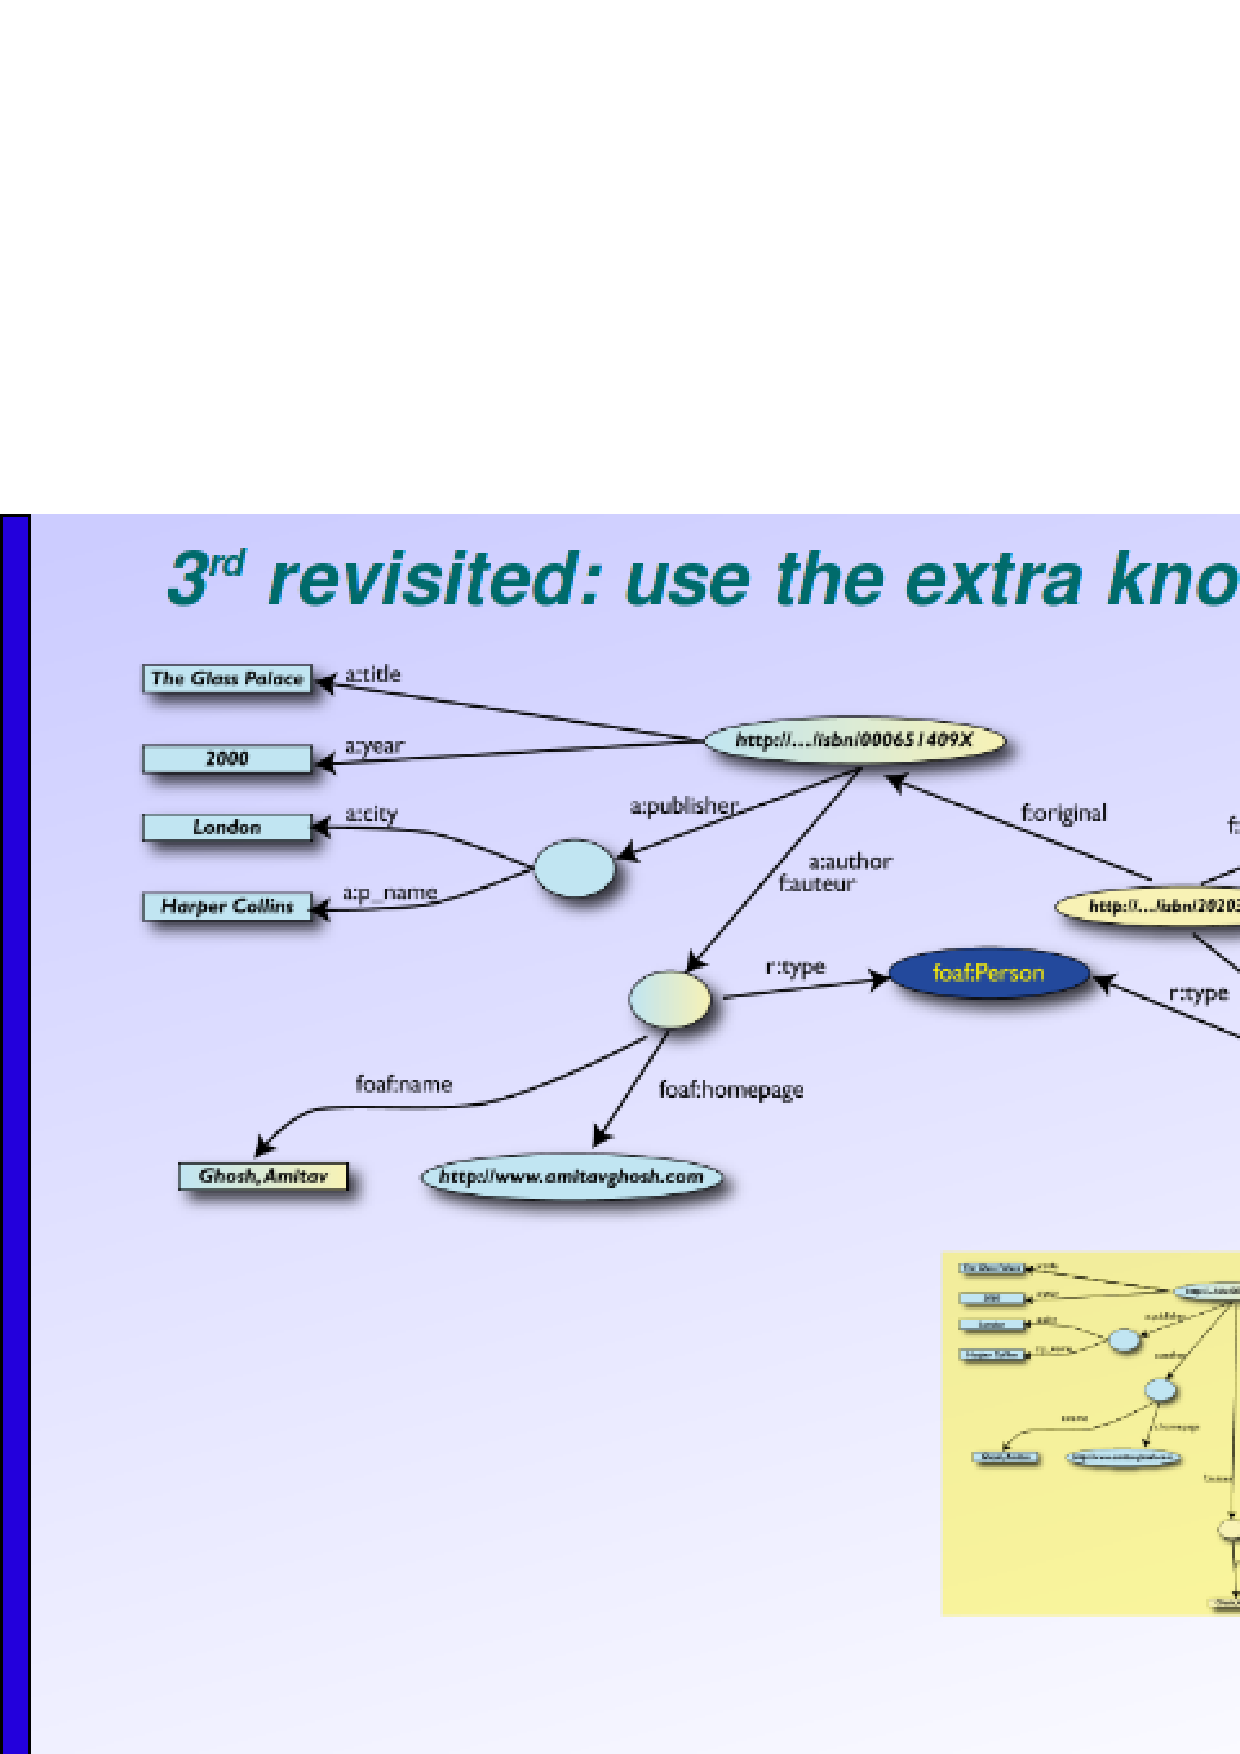
\includegraphics[width=0.9\textwidth]{../pics/img25.png}

\myslide{Start making richer queries!}

\begin{itemize}
\item User of dataset ``F'' can now query:
  \begin{itemize}
  \item ``donnes-moi la page d’accueil de l’auteur de l’originale''
  \item well… ``give me the home page of the original’s ‘auteur’''
  \end{itemize}
\item The information is not in datasets ``F'' or ``A
\item \ldots but was made available by:
  \begin{itemize}
  \item merging datasets ``A'' and datasets ``F''
  \item adding three simple extra statements as an extra ``glue''
  \end{itemize}
\end{itemize}

\myslide{Merge with Wikipedia Data}

\noindent
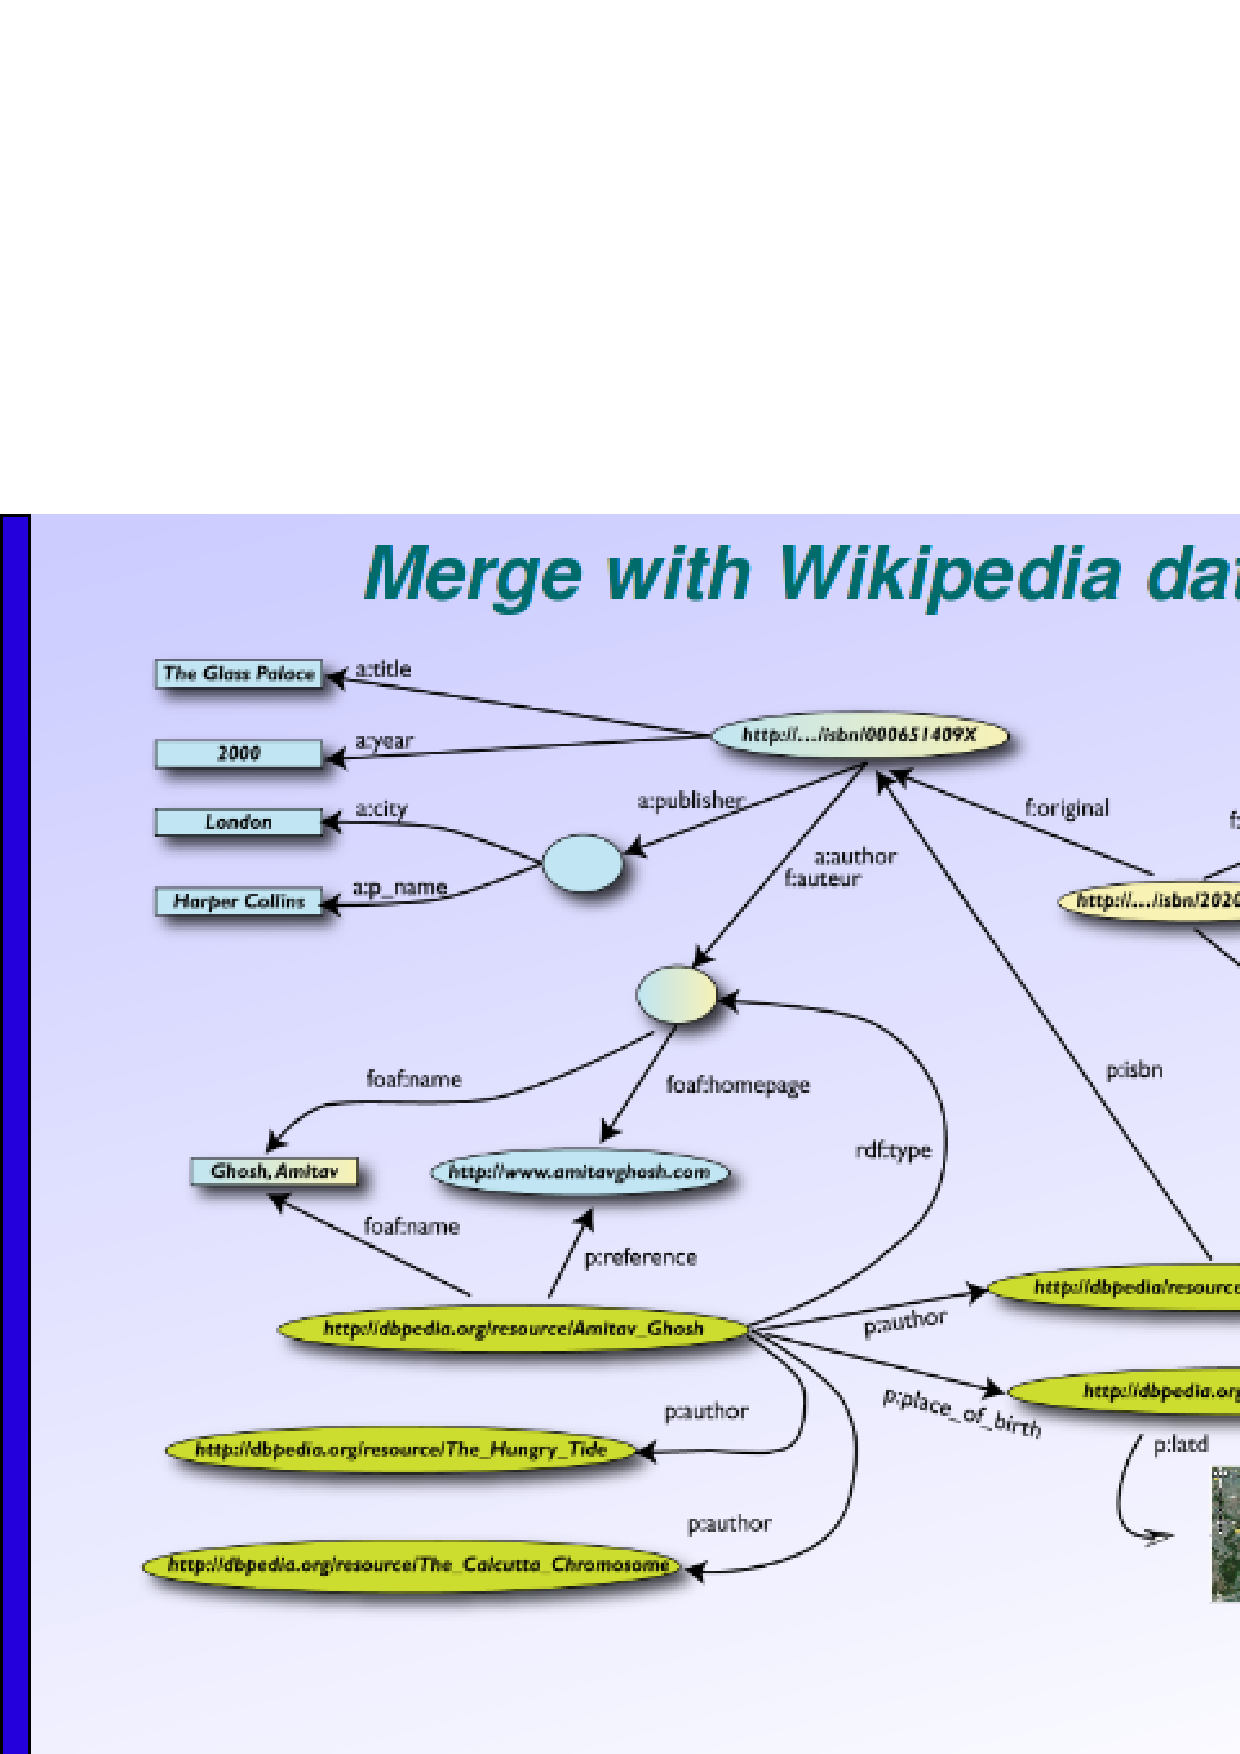
\includegraphics[width=0.9\textwidth]{../pics/img30.png}
\myslide{Merge with more Wikipedia Data}

\noindent
\includegraphics[width=0.9\textwidth]{../pics/img31.png}
% Is that surprising?

% \item Maybe but, in fact, no…
% \item What happened via automatic means is done all the time, every day by the users of the Web!
% \item The difference: a bit of extra rigour (e.g., naming the relationships) is necessary so that machines could do this, too

\myslide{What did we do?}

\begin{itemize}
\item We combined different datasets that
  \begin{itemize}
  \item are somewhere on the web
  \item are of different formats (mysql, excel sheet, XHTML, etc)
  \item have different names for relations
  \end{itemize}
\item We could combine the data because some URI-s were identical
  \\  (the ISBNs in this case)
\item We could add some simple additional information, using common terminologies that a community has produced
\item As a result, new relations could be found and retrieved
\end{itemize}

\myslide{It could become even more powerful}

\begin{itemize}
\item We could add extra knowledge to the merged datasets
  \begin{itemize}
  \item e.g., a full classification of various types of library data
  \item geographical information
  \item etc.
  \end{itemize}
\item This is where ontologies, extra rules, etc, come in
  \begin{itemize}
  \item ontologies/rule sets can be relatively simple and small, or huge, or anything in between…
  \end{itemize}
\item Even more powerful queries can be asked as a result!!!

\end{itemize}




\myslide{Criticism of the Semantic Web}
\MyLogo{\url{http://www.well.com/~doctorow/metacrap.htm} (lightly revised)}
Doctorow's seven insurmountable obstacles to reliable metadata are:
\begin{enumerate}
\item  People lie
\item  People are lazy
\item  People are stupid
\item  Mission Impossible: know thyself
\item  Schemas aren't neutral
\item  Metrics influence results
\item  There's more than one way to describe something
\end{enumerate}


\myslide{Cory Doctorow}
\MyLogo{https://xkcd.com/239/}

\includegraphics[width=0.9\textwidth]{../pics/blagofaire.png}

A Canadian-British blogger, journalist, and science fiction author who
serves as co-editor of the blog Boing Boing. He is an activist in
favour of liberalising copyright laws and a proponent of the Creative
Commons organization, using some of their licences for his books. Some
common themes of his work include digital rights management, file
sharing, and post-scarcity economics. (Wikipedia) 

\myslide{People lie}

Metadata exists in a competitive world. Suppliers compete to sell
their goods, cranks compete to convey their crackpot theories (mea
culpa), artists compete for audience.

Thus:
\begin{itemize}
\item    A search for any commonly referenced term at a search-engine like Altavista will often turn up at least one porn link in the first ten results.
\item     Your mailbox is full of spam with subject lines like "Re: The information you requested."
\item     Publisher's Clearing House sends out advertisements that holler "You may already be a winner!"
\item     Press-releases have gargantuan lists of empty buzzwords attached
\end{itemize}

\myslide{People are lazy}

Here in the Info-Ivory-Tower, we understand the importance of creating
and maintaining excellent metadata for our information.

But info-civilians are remarkably cavalier about their
information. Your clueless aunt sends you email with no subject line,
half the pages on Geocities are called "Please title this page" and
your boss stores all of his files on his desktop with helpful titles
like "UNTITLED.DOC."

\myslide{People are stupid}

Even when there's a positive benefit to creating good metadata, people
steadfastly refuse to exercise care and diligence in their metadata
creation.

Take eBay: every seller there has a damned good reason for
double-checking their listings for typos and misspellings. Try
searching for "plam" on eBay. Right now, that turns up nine typoed
listings for "Plam Pilots." Misspelled listings don't show up in
correctly-spelled searches and hence garner fewer bids and lower
sale-prices. You can almost always get a bargain on a Plam Pilot at
eBay.

The fine (and gross) points of literacy -- spelling, punctuation,
grammar -- elude the vast majority of the Internet's users. To believe
that J. Random Users will suddenly and en masse learn to spell and
punctuate -- let alone accurately categorize their information
according to whatever hierarchy they're supposed to be using -- is
self-delusion of the first water.

\myslide{Mission: Impossible -- know thyself}

In meta-utopia, everyone engaged in the heady business of describing
stuff carefully weighs the stuff in the balance and accurately divines
the stuff's properties, noting those results.

Simple observation demonstrates the fallacy of this assumption. When
Nielsen used log-books to gather information on the viewing habits of
their sample families, the results were heavily skewed to Masterpiece
Theater and Sesame Street. Replacing the journals with set-top boxes
that reported what the set was actually tuned to showed what the
average American family was really watching: light entertainment.

People are lousy observers of their own behaviors. Entire religions
are formed with the goal of helping people understand themselves
better; therapists rake in billions working for this very end.


\myslide{Schemas aren't neutral}

In a given sub-domain, say, Washing Machines, experts agree on
sub-hierarchies, with classes for reliability, energy consumption,
color, size, etc.

Nothing could be farther from the truth. Any hierarchy of ideas necessarily implies the importance of some axes over others. A manufacturer of small, environmentally conscious washing machines would draw a hierarchy that looks like this:
\begin{verbatim}
Energy consumption:
    Water consumption:
        Size:
            Capacity:
                Reliability

\end{verbatim}
\newpage
While a manufacturer of glitzy, feature-laden washing machines would want something like this:
\begin{verbatim}
Color:
    Size:
        Programmability:
            Reliability
\end{verbatim}

The conceit that competing interests can come to easy accord on a common vocabulary totally ignores the power of organizing principles in a marketplace.

\myslide{Metrics influence results}

Ranking axes are mutually exclusive: software that scores high for
security scores low for convenience, desserts that score high for
decadence score low for healthiness. Every player in a metadata
standards body wants to emphasize their high-scoring axes and
de-emphasize (or, if possible, ignore altogether) their low-scoring
axes.

It's wishful thinking to believe that a group of people competing to
advance their agendas will be universally pleased with any hierarchy
of knowledge. The best that we can hope for is a detente in which
everyone is equally miserable.

\myslide{There's more than one way to describe something}

"No, I'm not watching cartoons! It's cultural anthropology."

"This isn't smut, it's art."

"It's not plagiarism, it's borrowing!''

Reasonable people can disagree forever on how to describe something. Arguably, your Self is the collection of associations and descriptors you ascribe to ideas. Requiring everyone to use the same vocabulary to describe their material denudes the cognitive landscape, enforces homogeneity in ideas.

And that's just not right. 


\myslide{Other Issues}
\MyLogo{}
Other reasons that result in metadata becoming obsolete are:

\begin{enumerate}
\item Data may become irrelevant in time
\item Data may not be updated with new insights
\end{enumerate}

\textbf{Reliable Metadata}

\begin{itemize}
\item Information people \blu{use}
  \begin{itemize}
  \item Number of links into a page
  \item Text on the page
  \end{itemize}
\item Even this gets gamed (link farms, spam pages, \ldots)
\end{itemize}

\myslide{Semantic Web and NLP}

\begin{itemize}
\item The Semantic Web is about structuring data
\item Text Mining is about unstructured data
\item There is \blu{much more unstructured than structured data}
  \begin{itemize}
  \item NLP can infer structure
  \item NLP makes the Semantic Web feasible
  \item the Semantic Web can be a resource for NLP
  \end{itemize}
   (Computational) Linguistics is useful
%%% FIXME
% Examples

\end{itemize}

\myslide{Web 1.0/2.0/3.0}
\MyLogo{There's more than one way to describe something}

\begin{itemize}
\item[1.0] The \blu{read-only} web (1993--2001) 
  \\ interaction off-web (email, bulletin-boards, news-groups)
\item[2.0] The \blu{read/write/share} web (2001--2011) 
 \\ social media
\item[3.0] The \blu{personalized} web (2011--) 
\end{itemize}

The following pages are adapted from: CS Ramachandran (2011) ``Spinning the Web – 1.0, 2.0 or 3.0??''
In \textit{Blog:  Random Thoughts --- Thinking aloud about all things from Tech to life's bottlenecks}
July 11, 2011 \url{http://csramachandran.wordpress.com/2011/07/11/what-is-web3-0/} (accessed on 2011-03-26)

\myslide{Web 1.0}
\MyLogo{}
\begin{itemize} \addtolength{\itemsep}{-1.25ex}
\item  A \blu{read only} web
\item  A nascent internet space with around 250,000 websites
\item  Catering to 45 million users
\item  The era of Geocities \& Hotmail
\item  Dominated by Netscape and Internet Explorer browsers.
\item  It was all about read-only content and static HTML website
\item  Basic website design’s with Gif files
\item  Absence of dynamic user-generated content.
\end{itemize}

The era of Web 1.0 lasted from 1993 till the dot.com bubble burst in 2001.

\myslide{Web 2.0}
\begin{itemize} \addtolength{\itemsep}{-1.25ex}
\item  The \blu{read/write/share} web
\item  Rise of user-generated content
\item  Information sharing through blogs, social networks and image / video sites
\item  Enclyopedia Britannica replaced by Wikipedia
\item  Explosive growth of users – Over a billion users by 2006
\item  Brands and Websites start to focus on Social share and community buildings
\item  Emergence of Mobile Internet and Mobile Applications
\item  Rich User Experiences
\end{itemize}

\myslide{Web 3.0}
\MyLogo{Definition still in flux}
\begin{itemize} \addtolength{\itemsep}{-1.25ex}
\item  The \blu{personalized} web – iGoogle, My Yahoo, Personalized News Sites
\item  The \blu{ubiquitous} web: convergence of the virtual and physical world
\item  The \blu{semantic} Web – The web understands and anticipates requests
\item  The more you use the Web, the more your browser learns about you
\item  More localization of results – Google Places, Local Business Results
\item  Emergence of widgets and mashups (Combination of two applications – eg: review a place from Google Maps?)
\item  Behavioral targeting and advertising
\item  Evolution of a personal assistant who knows practically everything about you and your tastes
\item  More access points: computers, phones, cameras, TVs, \ldots
\end{itemize}



% \newpage
% \MyLogo{\shortstack{\url{http://msjosay.hubpages.com/hub/The-Difference-between-Web-20-and-Web-10}\\
%  \url{http://husseinahmed.com/2010/09/web-1-0-2-0-3-0-and-counting…/}}}
% 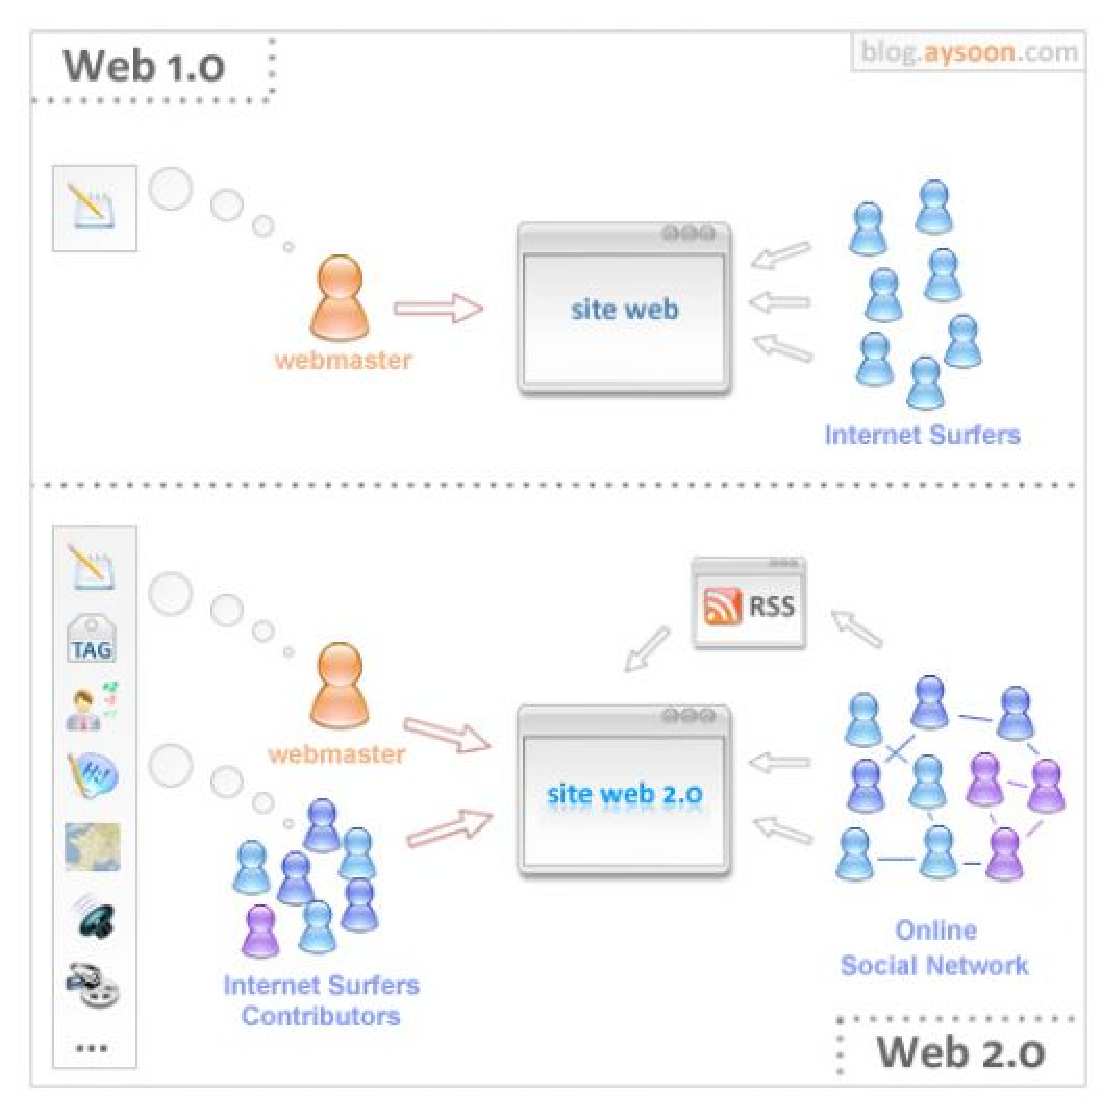
\includegraphics[height=\textheight]{../pics/web-2.0.eps}
% 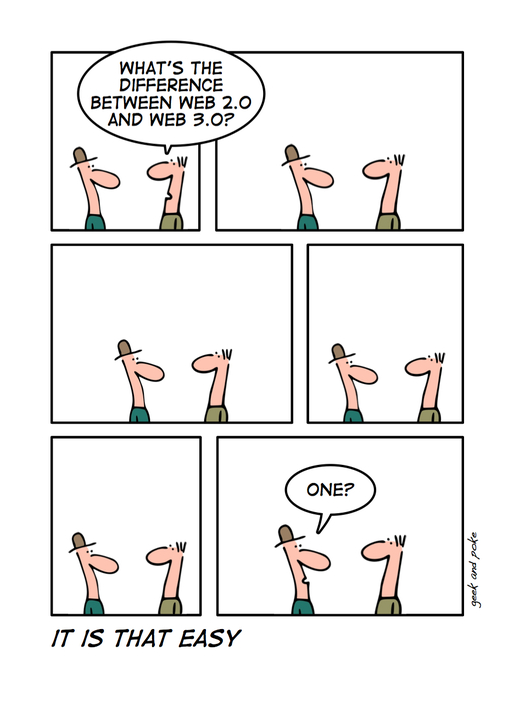
\includegraphics[height=\textheight]{../pics/web-3.0.eps}

% \myslide{Semantic Web Summary}


% \myslide{An example of why XML would be useful}


\myslide{Readings/Resources}
\MyLogo{}
\begin{itemize}
\item The Semantic Web and Ontologies
\\ \url{http://www.obitko.com/tutorials/ontologies-semantic-web/}
\item Criticism of the Semantic Web
\\ \url{http://www.well.com/~doctorow/metacrap.htm}
\item XML:  \url{http://en.wikipedia.org/wiki/XML}
\item Semantic Web in general: \url{semanticweb.org}
\item Nice presentation:  
\\ \url{http://www.w3.org/2004/Talks/0120-semweb-umich/}.
\end{itemize}

%I have taken slides from many of these.

\end{document}

%%% Local Variables: 
%%% coding: utf-8
%%% mode: latex
%%% TeX-PDF-mode: t
%%% TeX-engine: xetex
%%% End: 
